%\documentclass[10pt,dvipsnames]{beamer}
\documentclass[10pt,svgnames]{beamer}

\definecolor{links}{HTML}{2A1B81}
\hypersetup{colorlinks,linkcolor=,urlcolor=links}

\usetheme[numbering=fraction]{metropolis}
\metroset{block=fill}
%\setmonofont{Ubuntu Mono}

\usepackage{appendixnumberbeamer}

\usepackage{booktabs,empheq,bbold,bm}
\usepackage[scale=2]{ccicons}

\usepackage{pgfplots}
\usepackage{tikz}
\usetikzlibrary{math, positioning}

\usepgfplotslibrary{dateplot}

\usepackage{xspace}
\newcommand{\themename}{\textbf{\textsc{metropolis}}\xspace}

% for python listings; inspired by https://gist.github.com/YidongQIN/a10dd4f72381362aff4257e7a5541d86 
\usepackage{listings}
\usepackage{color}
\definecolor{darkred}{rgb}{0.6,0.0,0.0}
\definecolor{darkgreen}{rgb}{0,0.50,0}
\definecolor{lightblue}{rgb}{0.0,0.42,0.91}
\definecolor{orange}{rgb}{0.99,0.48,0.13}
\definecolor{grass}{rgb}{0.18,0.80,0.18}
\definecolor{pink}{rgb}{0.97,0.15,0.45}
\lstdefinelanguage{PythonPlus}[]{Python}{
  morekeywords=[1]{,as,assert,nonlocal,with,yield,self,True,False,None,} % Python builtin
  morekeywords=[2]{,__init__,__add__,__mul__,__div__,__sub__,__call__,__getitem__,__setitem__,__eq__,__ne__,__nonzero__,__rmul__,__radd__,__repr__,__str__,__get__,__truediv__,__pow__,__name__,__future__,__all__,}, % magic methods
  morekeywords=[3]{,object,type,isinstance,copy,deepcopy,zip,enumerate,reversed,list,set,len,dict,tuple,range,xrange,append,execfile,real,imag,reduce,str,repr,}, % common functions
  morekeywords=[4]{,Exception,NameError,IndexError,SyntaxError,TypeError,ValueError,OverflowError,ZeroDivisionError,}, % errors
  morekeywords=[5]{,ode,fsolve,sqrt,exp,sin,cos,arctan,arctan2,arccos,pi, array,norm,solve,dot,arange,isscalar,max,sum,flatten,shape,reshape,find,any,all,abs,plot,linspace,legend,quad,polyval,polyfit,hstack,concatenate,vstack,column_stack,empty,zeros,ones,rand,vander,grid,pcolor,eig,eigs,eigvals,svd,qr,tan,det,logspace,roll,min,mean,cumsum,cumprod,diff,vectorize,lstsq,cla,eye,xlabel,ylabel,squeeze,}, % numpy / math
}
\lstdefinestyle{colorEX}{
  basicstyle=\ttfamily\small,
  backgroundcolor=\color{white},
  commentstyle=\color{darkgreen}\slshape,
  keywordstyle=\color{blue}\bfseries\itshape,
  keywordstyle=[2]\color{blue}\bfseries,
  keywordstyle=[3]\color{grass},
  keywordstyle=[4]\color{red},
  keywordstyle=[5]\color{orange},
  stringstyle=\color{darkred},
  emphstyle=\color{pink}\underbar,
}
\lstset{style=colorEX,
        basewidth = {.49em}}

\newtheorem*{conjecture}{Conjecture}
\newtheorem*{cproblem}{continuum problem}

\newcommand{\bg}{\mathbf{g}}
\newcommand{\bn}{\mathbf{n}}
\newcommand{\bq}{\mathbf{q}}
\newcommand{\bu}{\mathbf{u}}

\newcommand{\bU}{\mathbf{U}}

\newcommand{\bzero}{\bm{0}}

\newcommand{\cK}{\mathcal{K}}
\newcommand{\cV}{\mathcal{V}}
\newcommand{\cX}{\mathcal{X}}

\newcommand{\RR}{\mathbb{R}}

\newcommand{\nn}{\mathrm{n}}
\newcommand{\pp}{\mathrm{p}}
\newcommand{\qq}{\mathrm{q}}
\newcommand{\rr}{\mathrm{r}}

\newcommand{\eps}{\epsilon}
\newcommand{\grad}{\nabla}
\newcommand{\Div}{\nabla\cdot}

\newcommand{\rhoi}{\rho_{\text{i}}}
\newcommand{\snew}{s^{\text{new}}}

\newcommand{\sdoi}[1]{\,{\scriptsize \href{https://doi.org/#1}{doi:#1}}}
\newcommand{\surl}[2]{\,{\scriptsize \href{#1}{#2}}}

\newcommand{\comm}[1]{{\footnotesize \hfill \emph{#1}}}
\newcommand{\where}[1]{\text{\footnotesize #1}}
\newcommand{\viewin}[1]{{\footnotesize \emph{this view appears in} #1}}

\renewcommand*{\thefootnote}{\fnsymbol{footnote}}

\newcommand{\aler}[1]{{\color{FireBrick} #1}}


\title{Surface elevation errors in finite element \\ Stokes models for glacier evolution}

\date{Numerical Analysis Seminar, Stockholm University (September 2025)}

\author{Ed Bueler, University of Alaska Fairbanks}

\titlegraphic{\vspace{-1cm}\par\hspace{-1cm}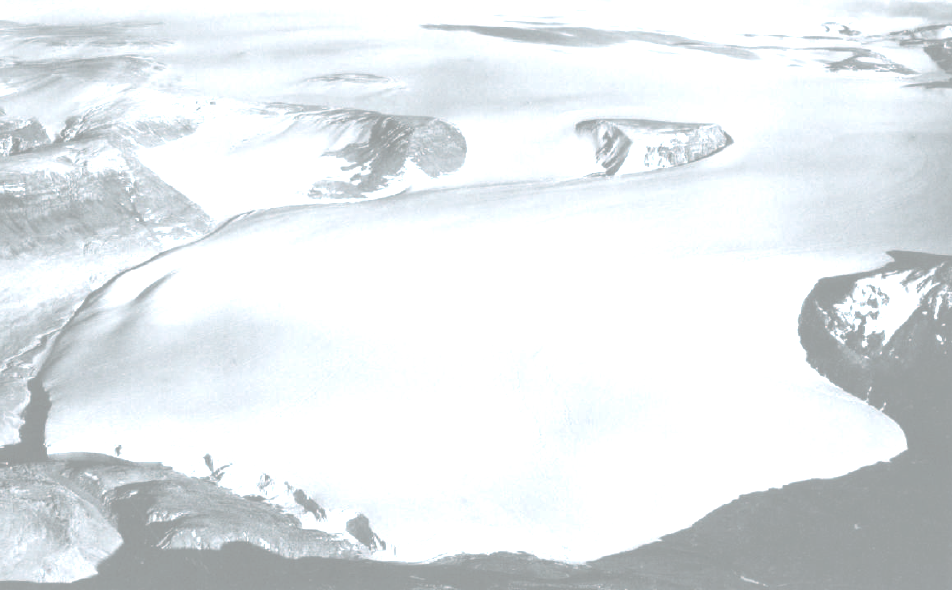
\includegraphics[width=1.5\textwidth]{figs/polaris-overexposed.png}%

\vspace{-25mm}
\hfill 
\includegraphics[width=0.2\textwidth]{figs/uafbw.png}}

\begin{document}
\graphicspath{{figs/}{../../paper/figs/}}

\maketitle


\begin{frame}[plain]

\mbox{\hspace{-9mm} 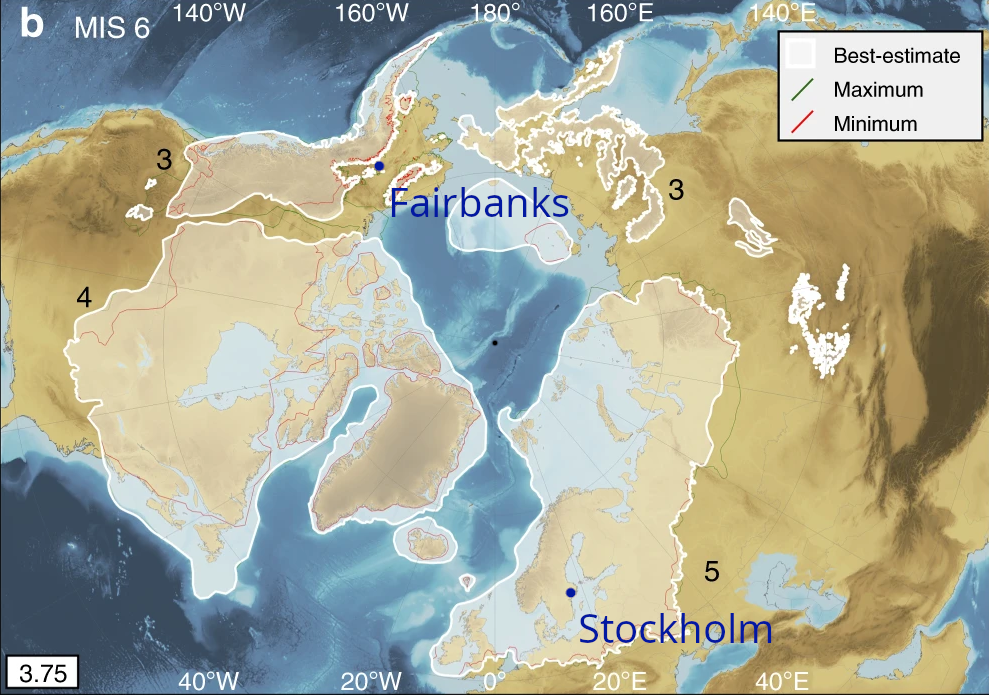
\includegraphics[width=1.15\textwidth]{nhsheets.png}}

\vspace{-2mm}
\hfill {\tiny Fig.~1 from Batchelor (2019), \emph{The configuration of Northern Hemisphere ice sheets through the Quaternary}}
\end{frame}


\begin{frame}{the ``extent of glaciation'' question}

\begin{itemize}
\item \alert{where are there glaciers?}
\item that is, in a given climate and with a given topography, what is the extent of glaciation?  what is the geometry of those glaciers?
\item this is my motivation for numerically solving the free-boundary problem for the surface elevation functions of glaciers
\end{itemize}
\end{frame}


\begin{frame}{Outline}
  \setbeamertemplate{section in toc}[sections numbered]
  \tableofcontents[hideallsubsections]
\end{frame}

\AtBeginSection[]
{% do not put toc here this time
}


\section{variational inequalities (VIs)}

\begin{frame}{reminder: coercivity for gradients}

\begin{itemize}
\item to start, let's recall a famous inequality from convex optimization
\item let $J: \RR^n \to \RR$ be a smooth objective function
\item suppose Hessian $H_J$ is uniformly symmetric positive definite (SPD)
    \begin{itemize}
    \item[$\circ$] thus $J$ is convex
    \end{itemize}
\end{itemize}

\bigskip
\begin{theorem}
the gradient $F=\nabla J$ is \aler{coercive}: there exists $\alpha > 0$ so that
$$(F(x) - F(y)) \cdot (x - y) \ge \alpha \|x - y\|^2$$
\end{theorem}

\smallskip
\emph{Proof.} By Taylor expansion, and $H_J \ge \alpha I$ with $\alpha=\lambda_{\text{min}}(H_J(x))$,
\begin{align*}
J(x) - J(y) &\ge F(y) \cdot (x - y) + \frac{\alpha}{2} \|y-x\|^2 \\
J(y) - J(x) &\ge F(x) \cdot (y - x) + \frac{\alpha}{2} \|y-x\|^2
\end{align*}
Add: \quad $0 \ge (F(y) - F(x)) \cdot (x-y) +  \alpha \|x - y\|^2$. \qed
\end{frame}


\begin{frame}{example of a variational inequality: classical obstacle problem}

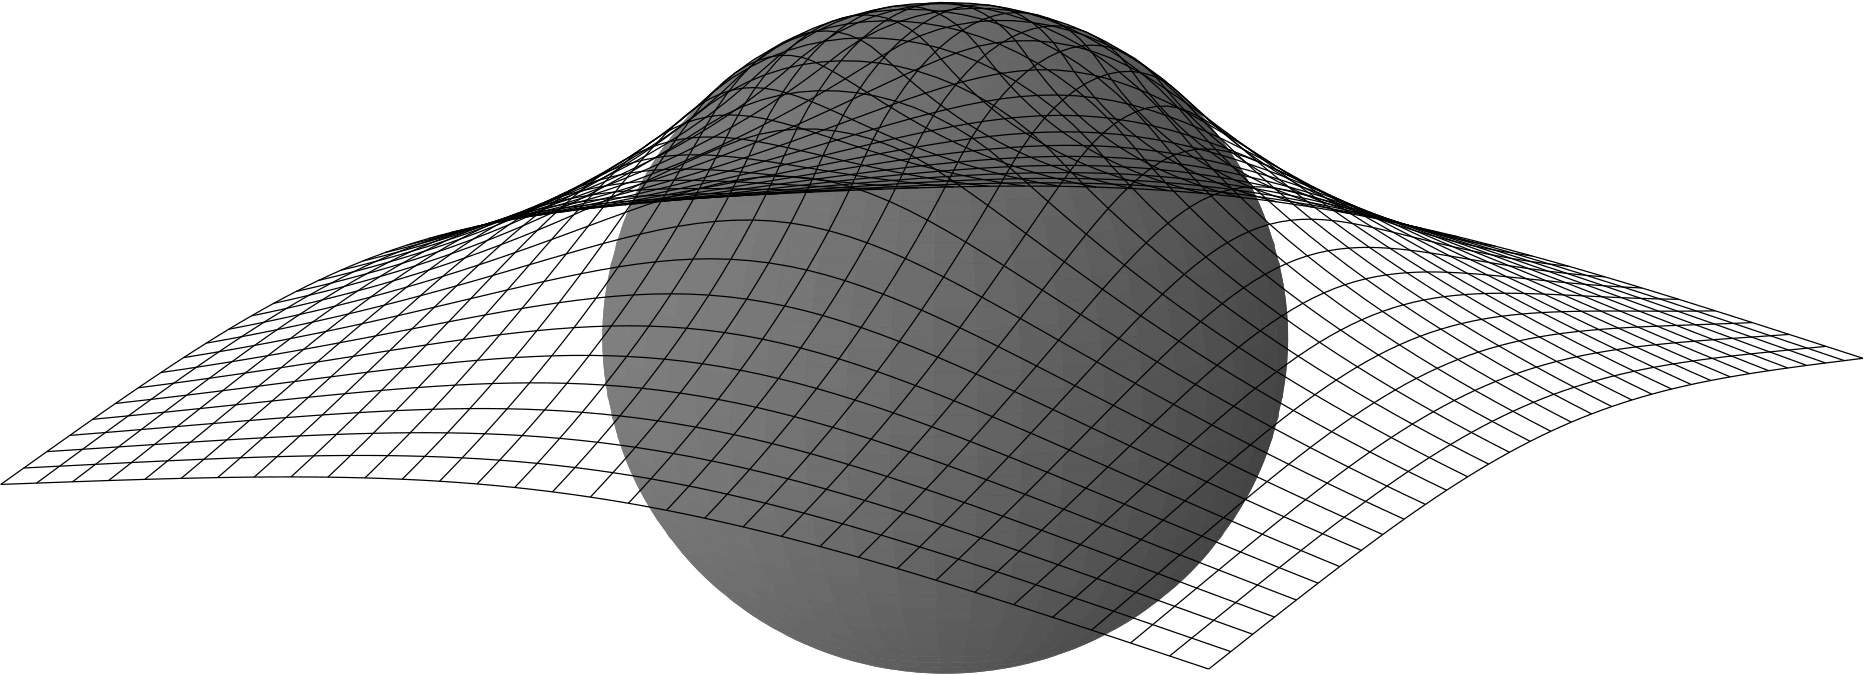
\includegraphics[width=0.55\textwidth]{figs/obstacle65.png} \qquad 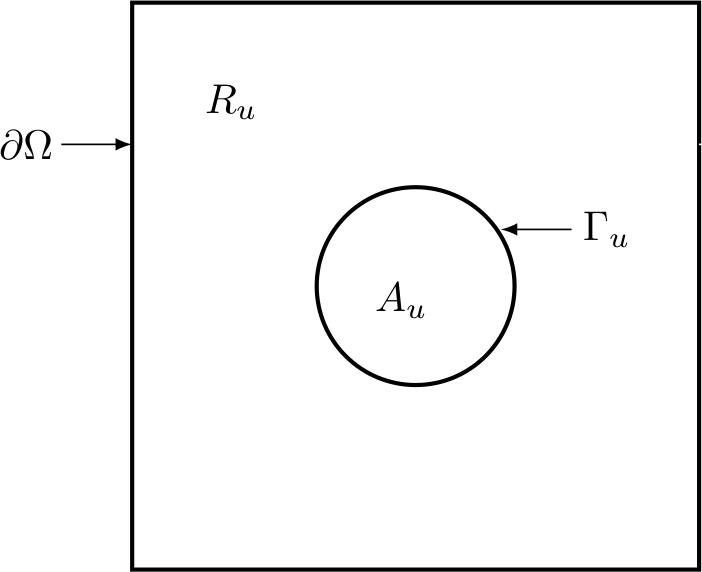
\includegraphics[width=0.35\textwidth]{figs/obstacle-sets.png}

\only<1>{
\begin{itemize}
\item given: domain $\Omega\subset \RR^2$, obstacle $\psi$, Dirichlet condition $g$, source $\varphi$
\item define \emph{admissible set}: \, $\cK = \left\{v \in H^1(\Omega) \,:\, v\big|_{\partial \Omega} = g \text{ and } v \ge \psi\right\}$
\item the \emph{\aler{variational inequality}} (VI) is to find $u\in\cK$ so that
    $$\int_\Omega \grad u\cdot \grad (v-u) - \varphi (v-u) \ge 0 \quad \text{for all } v \in \cK$$
\end{itemize}
}
\only<2>{
\begin{itemize}
\item the solution defines \emph{\aler{active}} $A_u = \{u = \psi\}$ and \emph{\aler{inactive}} $R_u = \{u> \psi\}$ subsets of $\Omega$, and a \emph{\aler{free boundary}} $\Gamma_u=\partial R_u \cap \Omega$
\item naive strong form poses the problem in terms of its solution?:
\begin{align*}
-\grad^2 u &= \varphi \quad \text{ on $R_u$} \\
u &= \psi \quad \text{ on $A_u$}
\end{align*}
\end{itemize}
}
\end{frame}


\begin{frame}{general variational inequalities}

\begin{itemize}
\item let $\cV$ be a real, reflexive Banach space
\item let $\cK \subset \cV$ be a closed and convex subset
\item suppose $F:\cK \to \cV'$ is a continuous, generally nonlinear operator
    \begin{itemize}
    \item[$\circ$] $F$ may be defined \emph{only} on $\mathcal{K}$
    \item[$\circ$] $F$ may \emph{not}\, be the derivative of an objective function $J$
    \end{itemize}
\item the general variational inequality problem {\color{FireBrick} VI($F$,$\mathcal{K}$)} is
	$${\color{FireBrick} F(u)[v-u] \ge 0 \quad \text{ for all } v \in \mathcal{K}}$$
\item when $\mathcal{K}$ is nontrivial, VI($F$,$\mathcal{K}$) is nonlinear 
    \begin{itemize}
    \item[$\circ$] even when $F$ is a linear operator
    \item[$\circ$] classical problem has linear operator: \, $F(v)[w] = \int_\Omega \grad v\cdot \grad w - \varphi w$
    \end{itemize}
\end{itemize}
\end{frame}


\begin{frame}{VI $=$ ``constrained equation''}

\begin{center}
\begin{tabular}{l|l}
\begin{minipage}[t][16mm][t]{0.4\textwidth}
unconstrained optimization:
$$\min_{u\in\mathcal{V}} J(u)$$
\end{minipage}
&
\begin{minipage}[t][16mm][t]{0.4\textwidth}
constrained optimization:
$$\min_{u\in\mathcal{K}} J(u)$$
\end{minipage}
\\ \hline
\begin{minipage}[t][16mm][t]{0.4\textwidth}
equation for $u \in \mathcal{V}$: {\LARGE \strut}

$$F(u)=0$$
\end{minipage}
&
\begin{minipage}[t][16mm][t]{0.4\textwidth}

\vspace{-2mm}
{\color{FireBrick} VI} for $u \in \mathcal{K}$:
$${\color{FireBrick} F(u)[v-u] \ge 0 \quad \forall v \in \mathcal{K}}$$
\end{minipage}
\end{tabular}
\end{center}
\end{frame}


\begin{frame}{FIXME}

FIXME  $q$-coercivity gives well-posedness
\end{frame}


\section{a new \emph{a priori} error bound for VIs}

\begin{frame}{FIXME}

FIXME
\end{frame}


\section{the standard glacier model}

\begin{frame}{glacier evolution in space-time \only<2>{ \dots implicitly?}}

\bigskip \bigskip

\begin{columns}
\begin{column}{0.28\textwidth}
\begin{itemize}
\item[a)] what is true within the {\color{RoyalBlue} ice}?
\item[b)] what is true on {\color{OliveDrab} bare land}?
\item[c)] what is true on {\color{Salmon} free boundary}?
\end{itemize}\end{column}
\begin{column}{0.72\textwidth}
FIXME %\only<1>{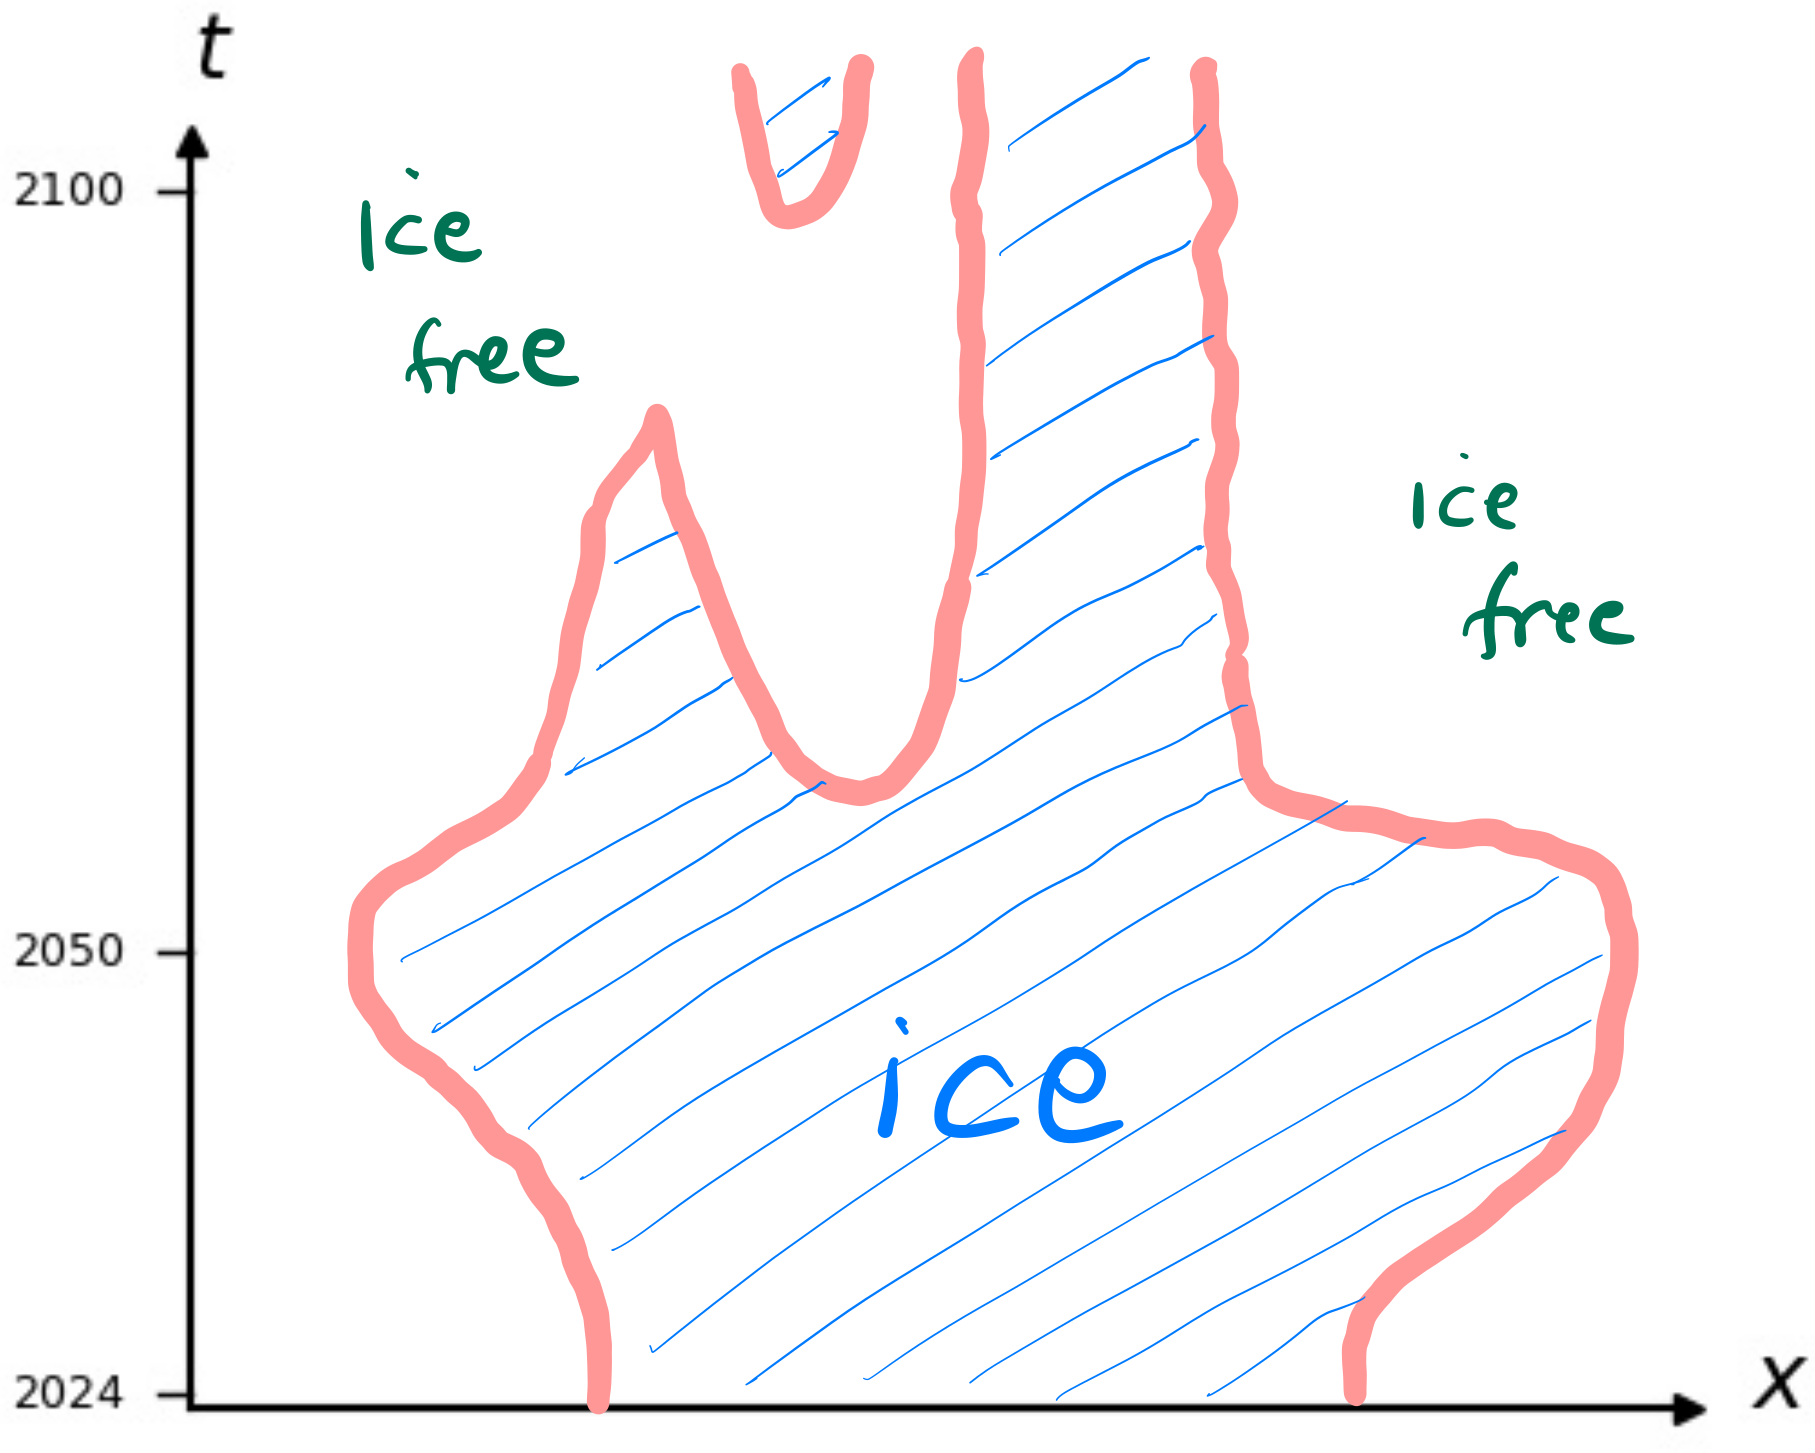
\includegraphics[height=65mm]{xtcrop}}\only<2>{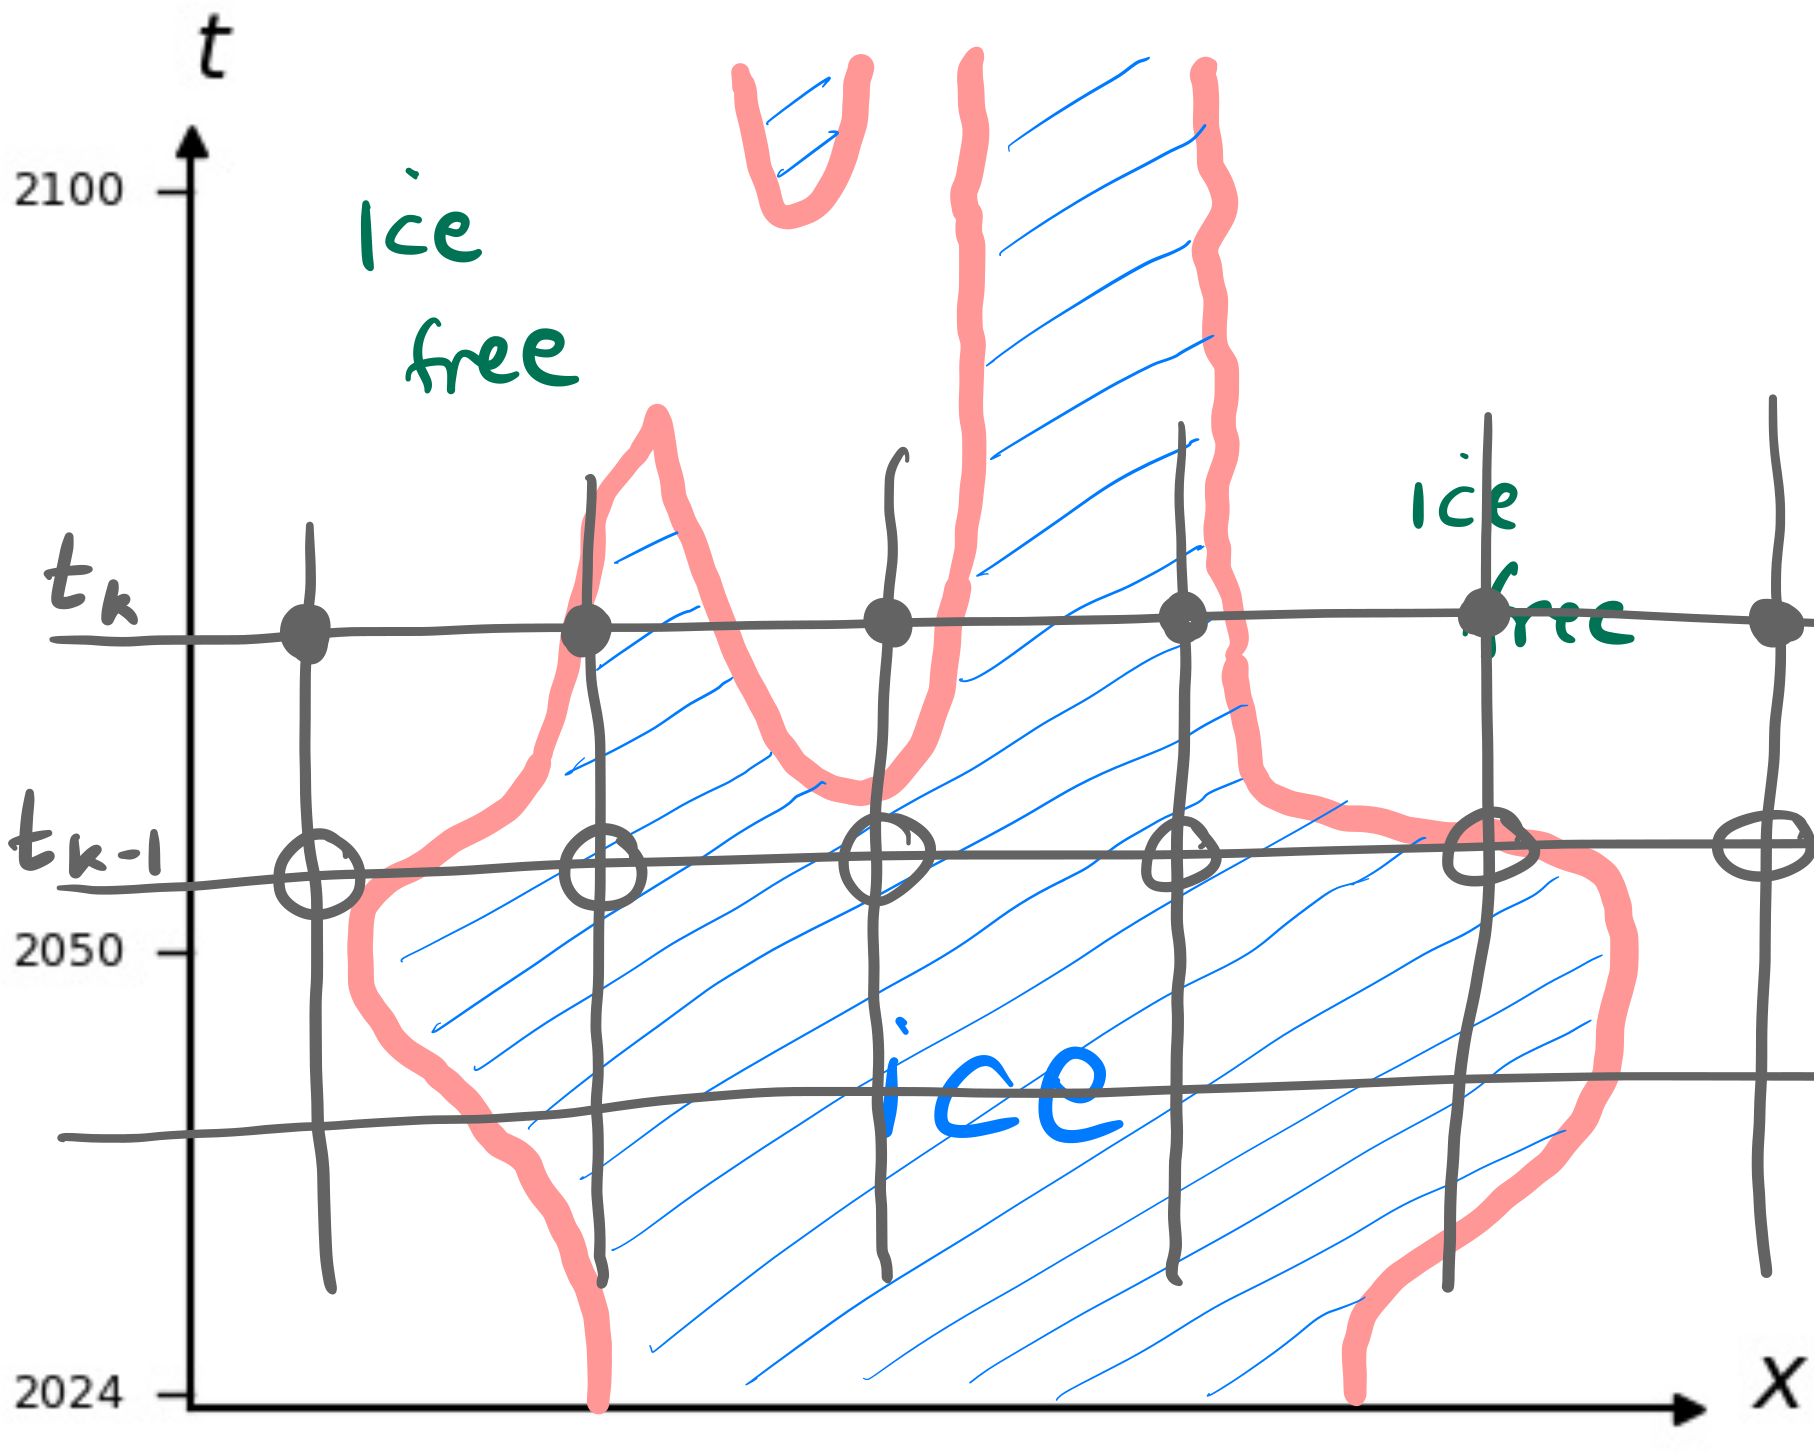
\includegraphics[height=65mm]{implicitstep}}
\end{column}
\end{columns}
\end{frame}

\begin{frame}{the 3 views}

\vspace{-2mm}
\begin{center}
FIXME %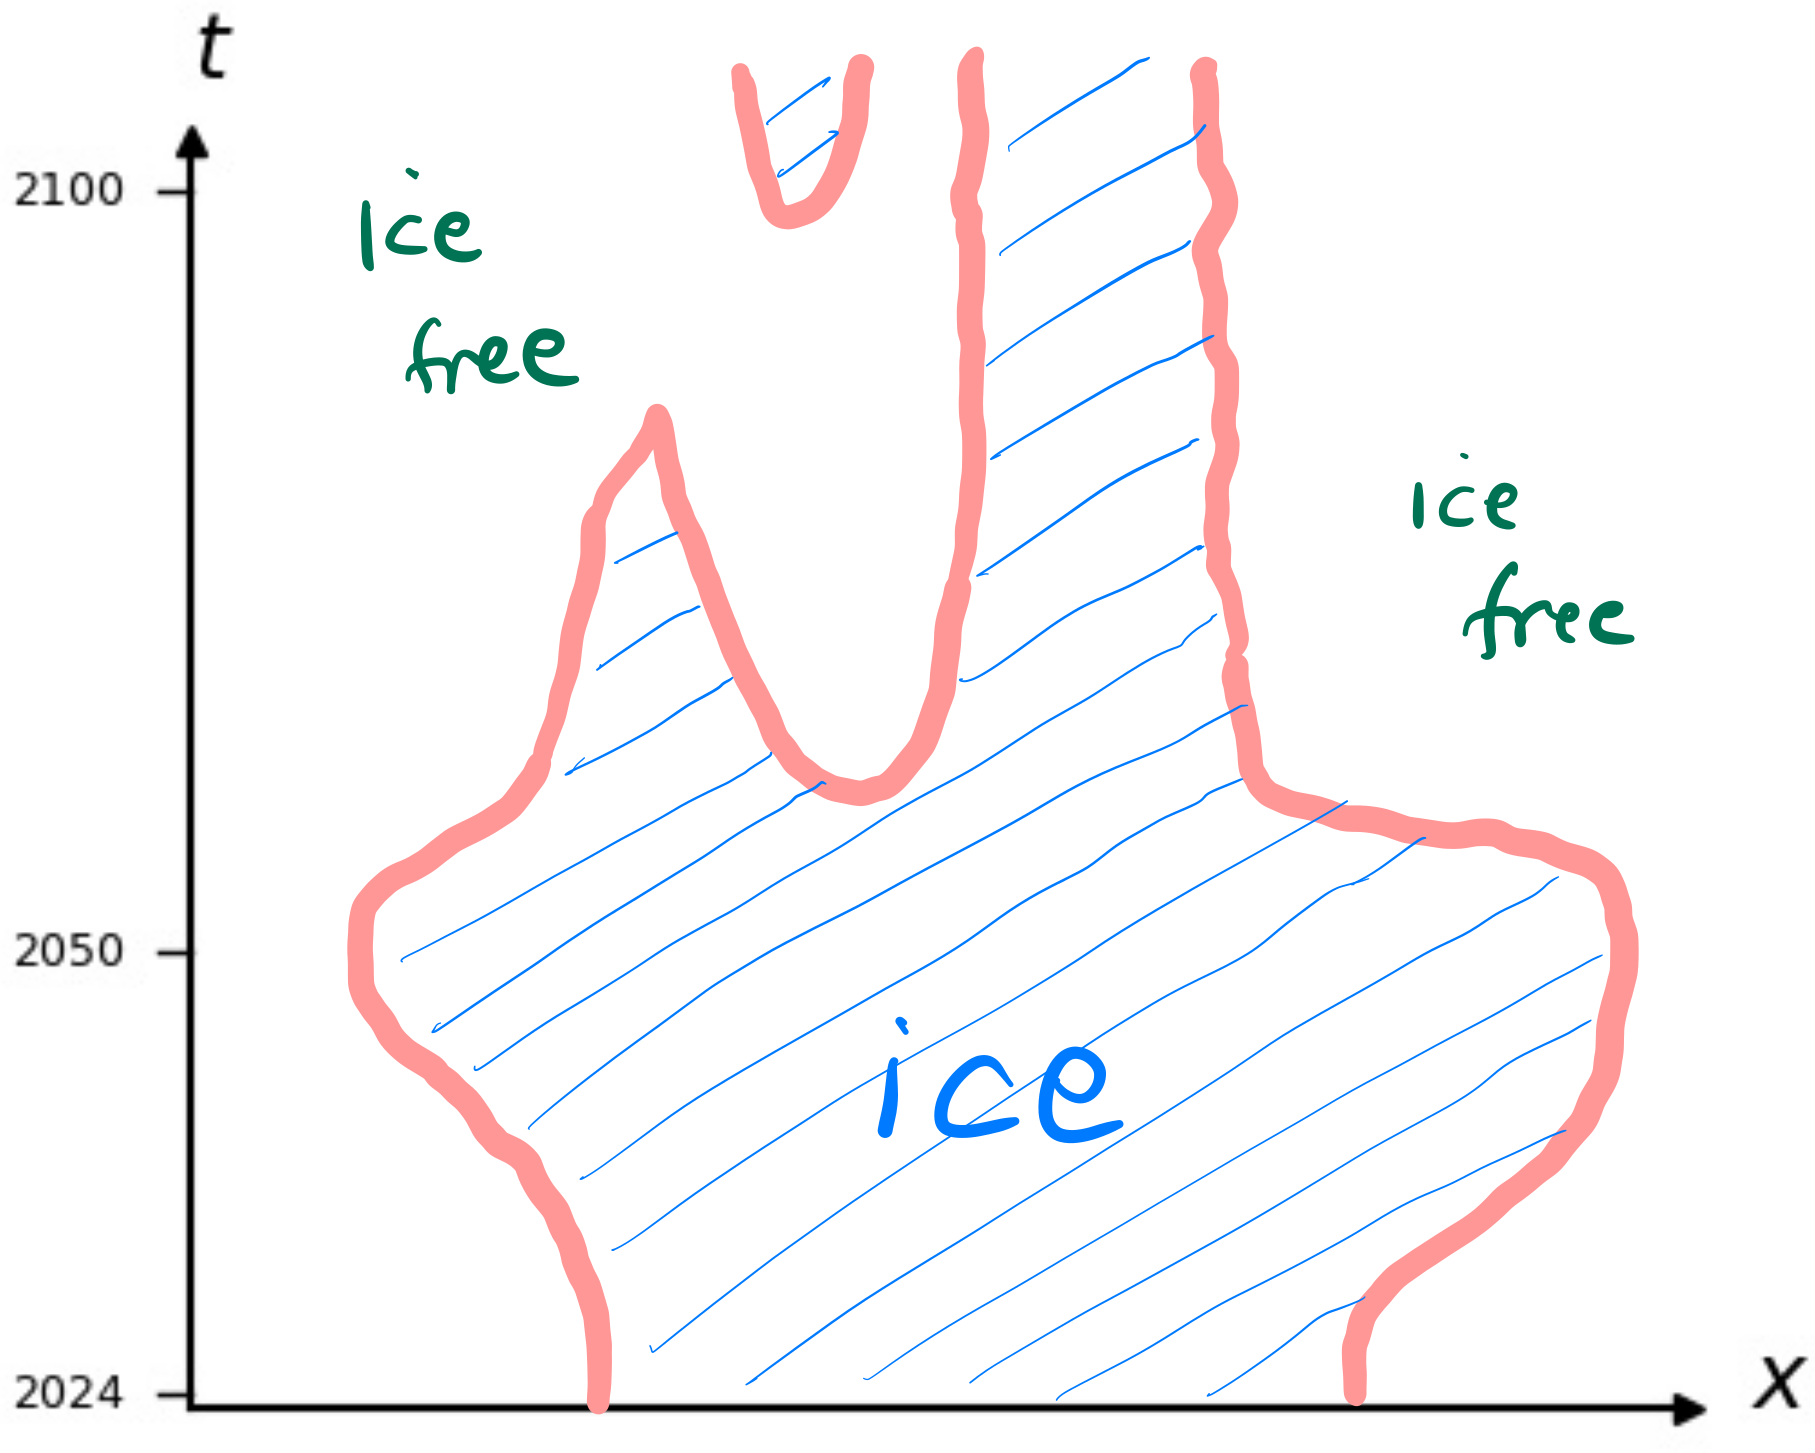
\includegraphics[width=0.55\textwidth]{xtcrop}
\end{center}

\vspace{-2mm}
\begin{columns}
\begin{column}{0.43\textwidth}
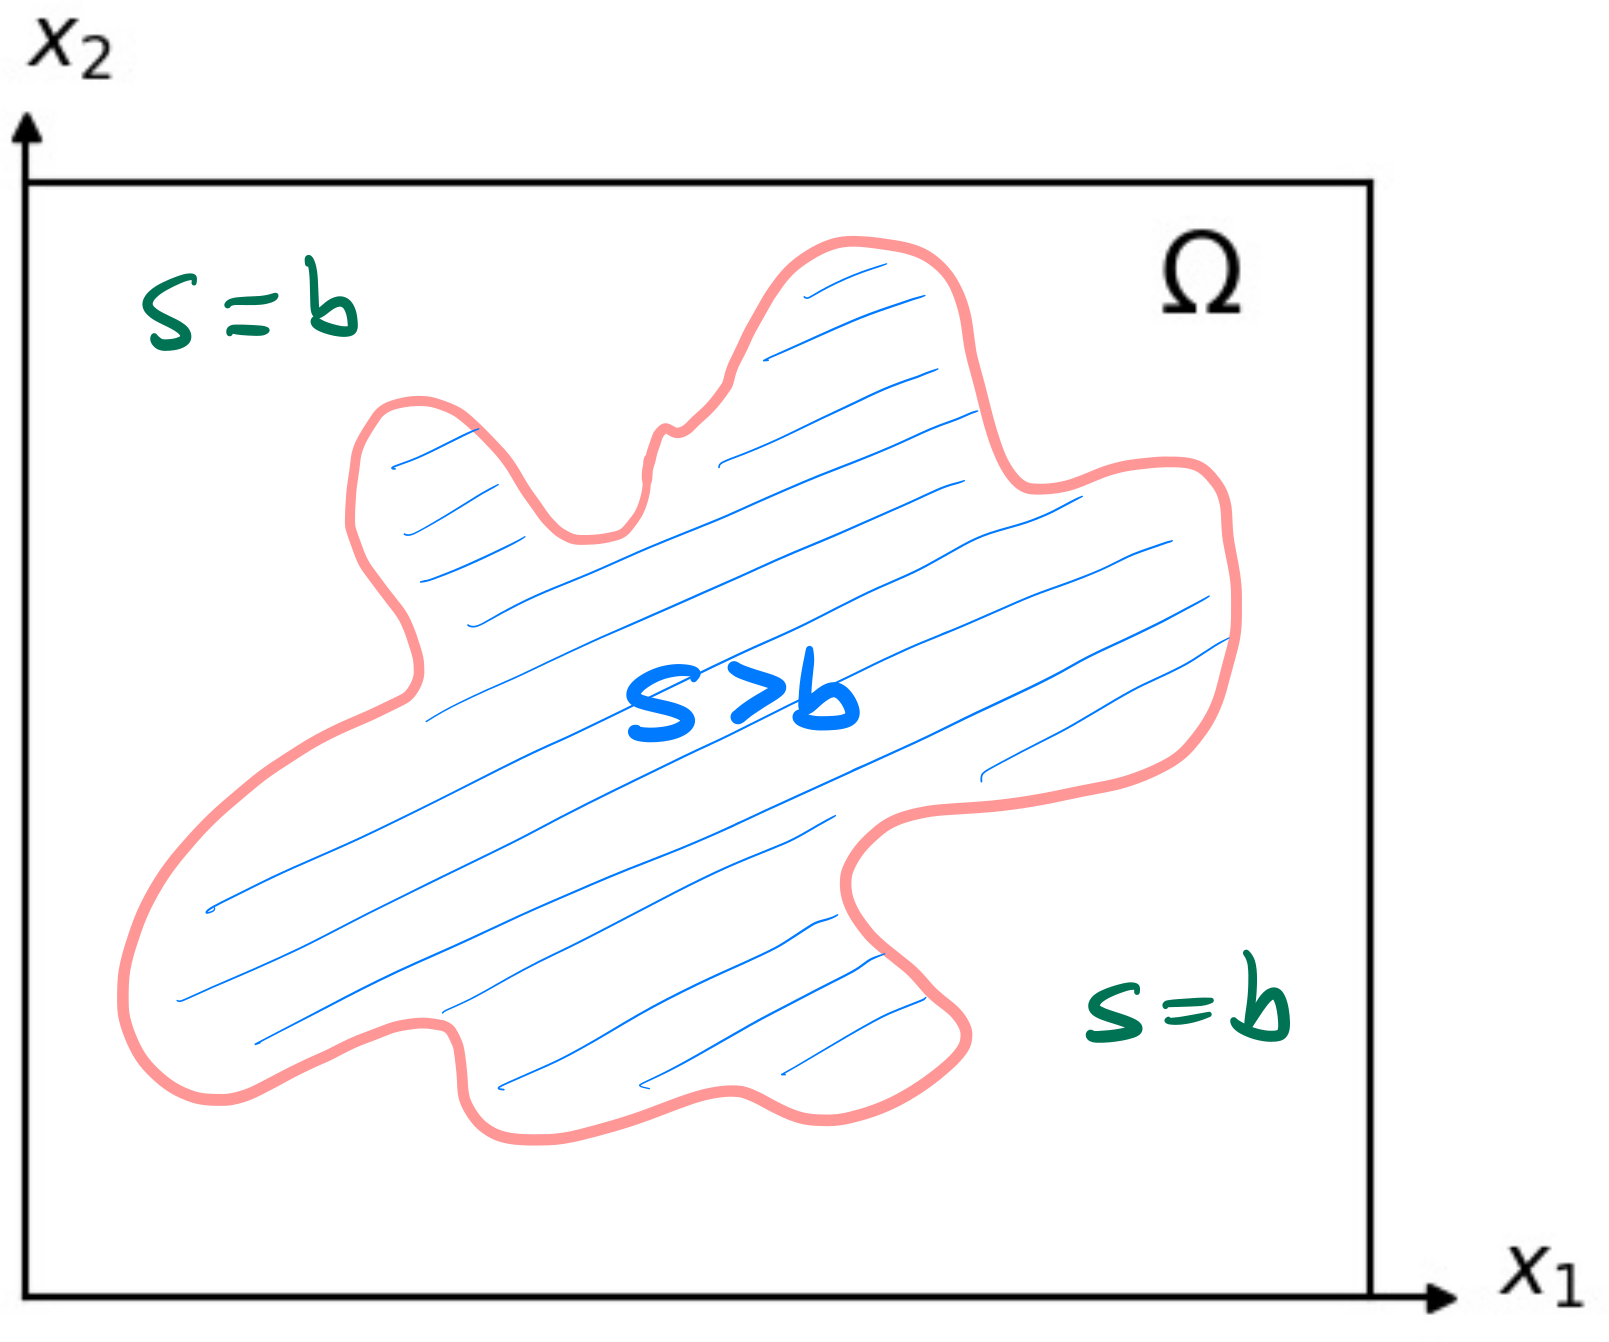
\includegraphics[width=0.9\textwidth]{mapplane}
\end{column}
\begin{column}{0.57\textwidth}
FIXME %\hfill 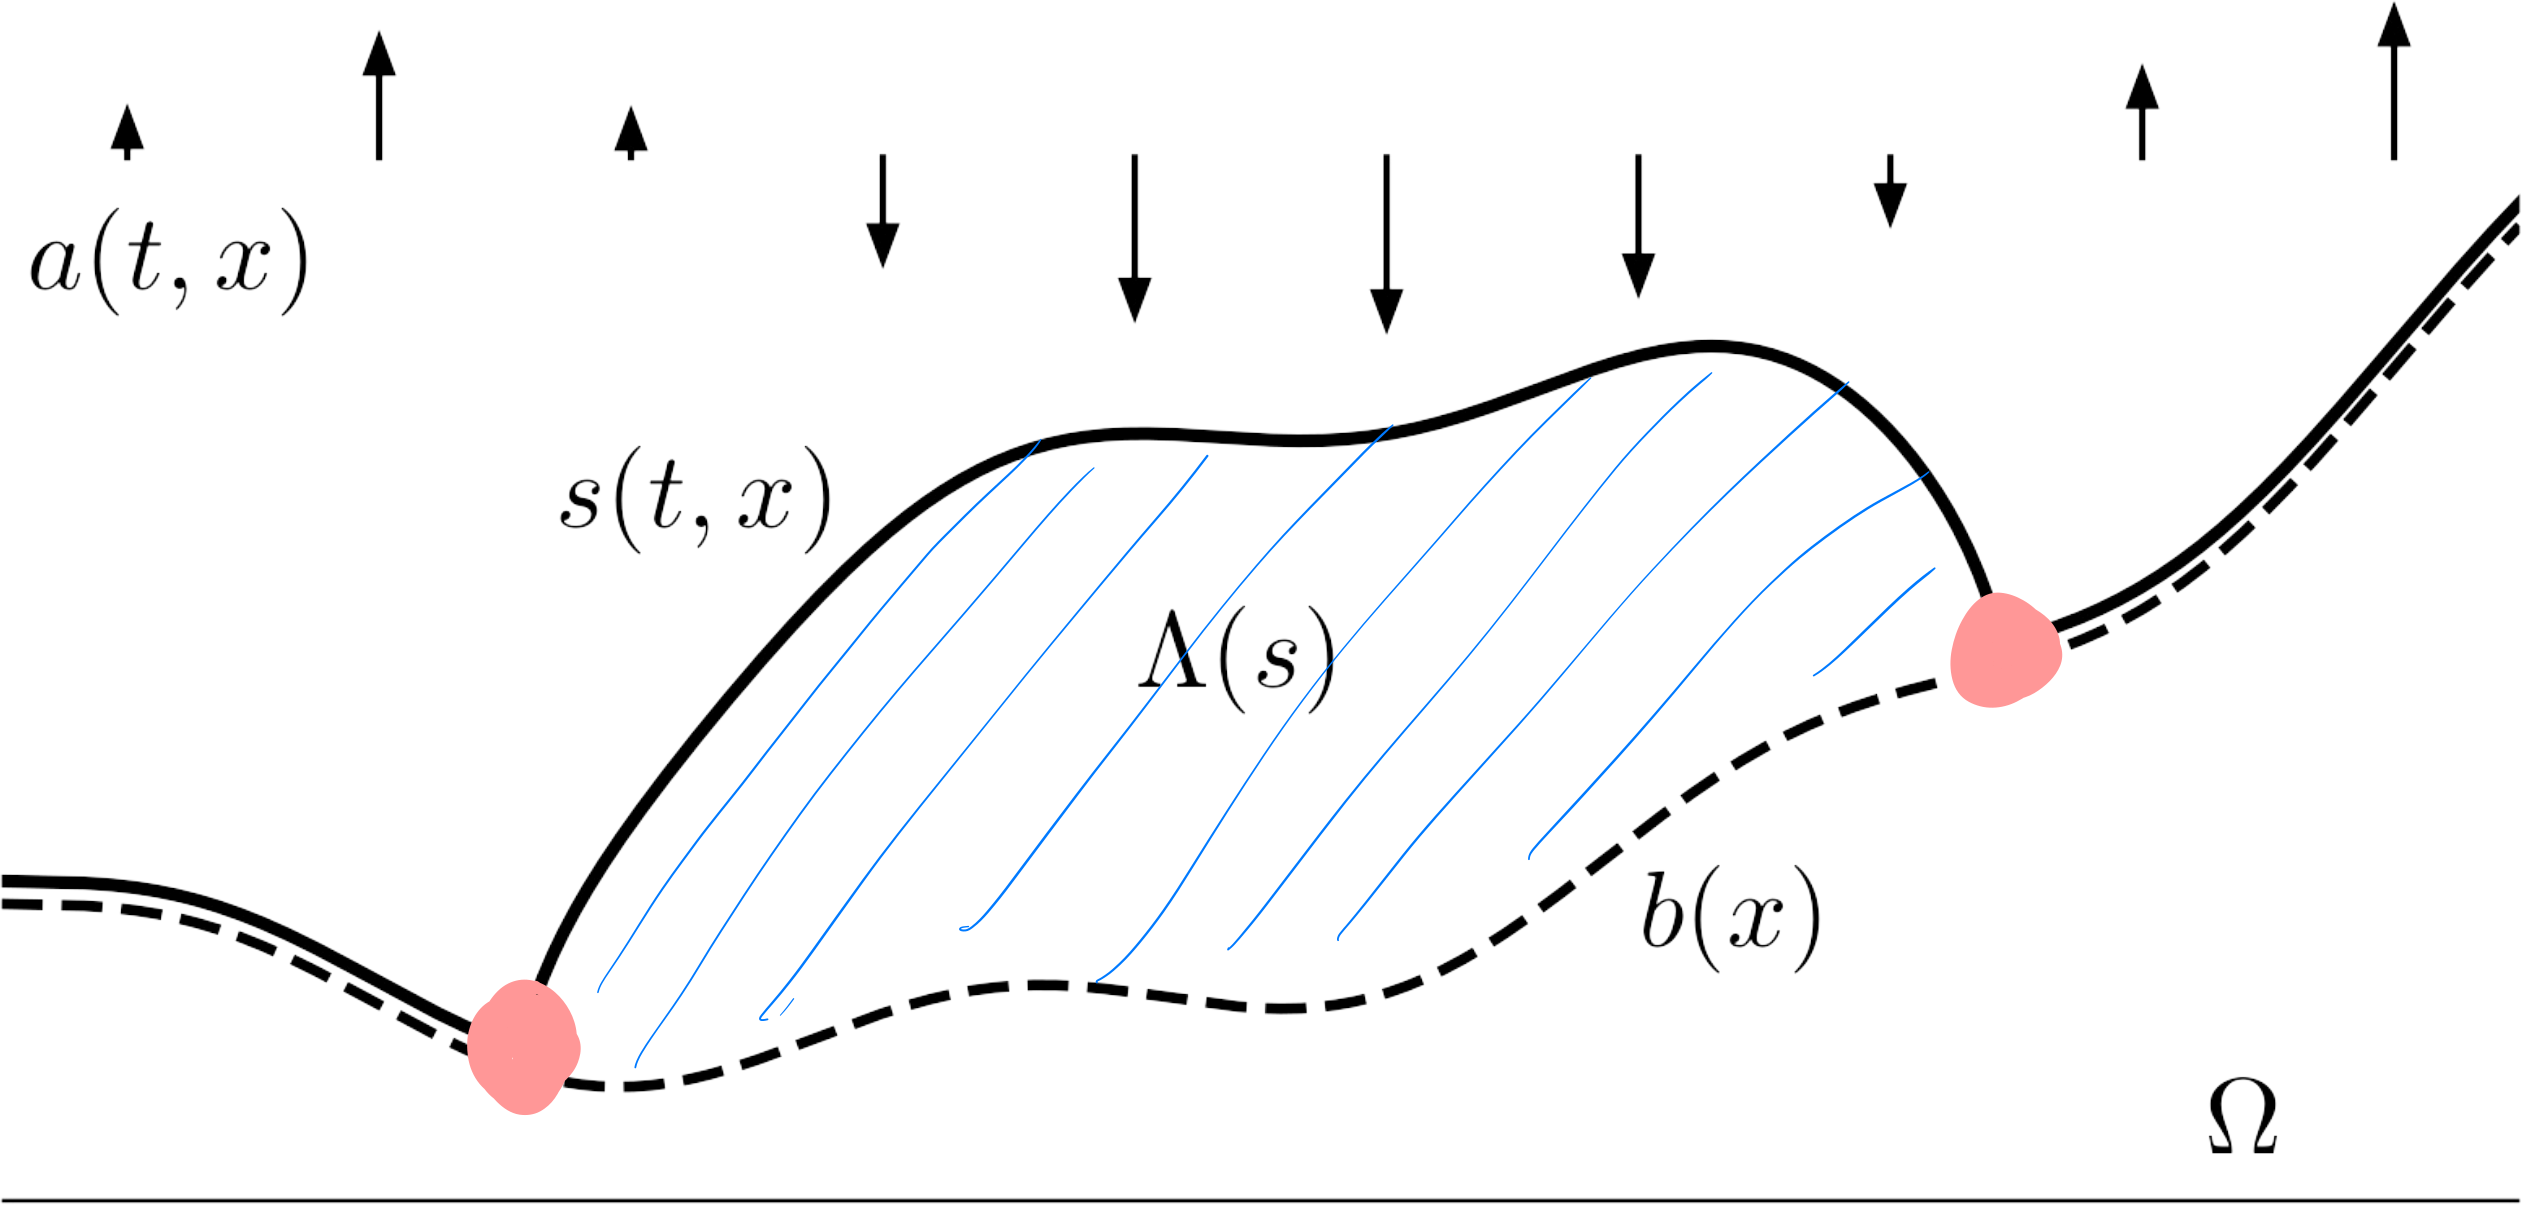
\includegraphics[width=\textwidth]{stokesdomainOmega}
\end{column}
\end{columns}
\end{frame}


\begin{frame}{what is true everywhere in $[0,T]\times\Omega$?}

\hfill 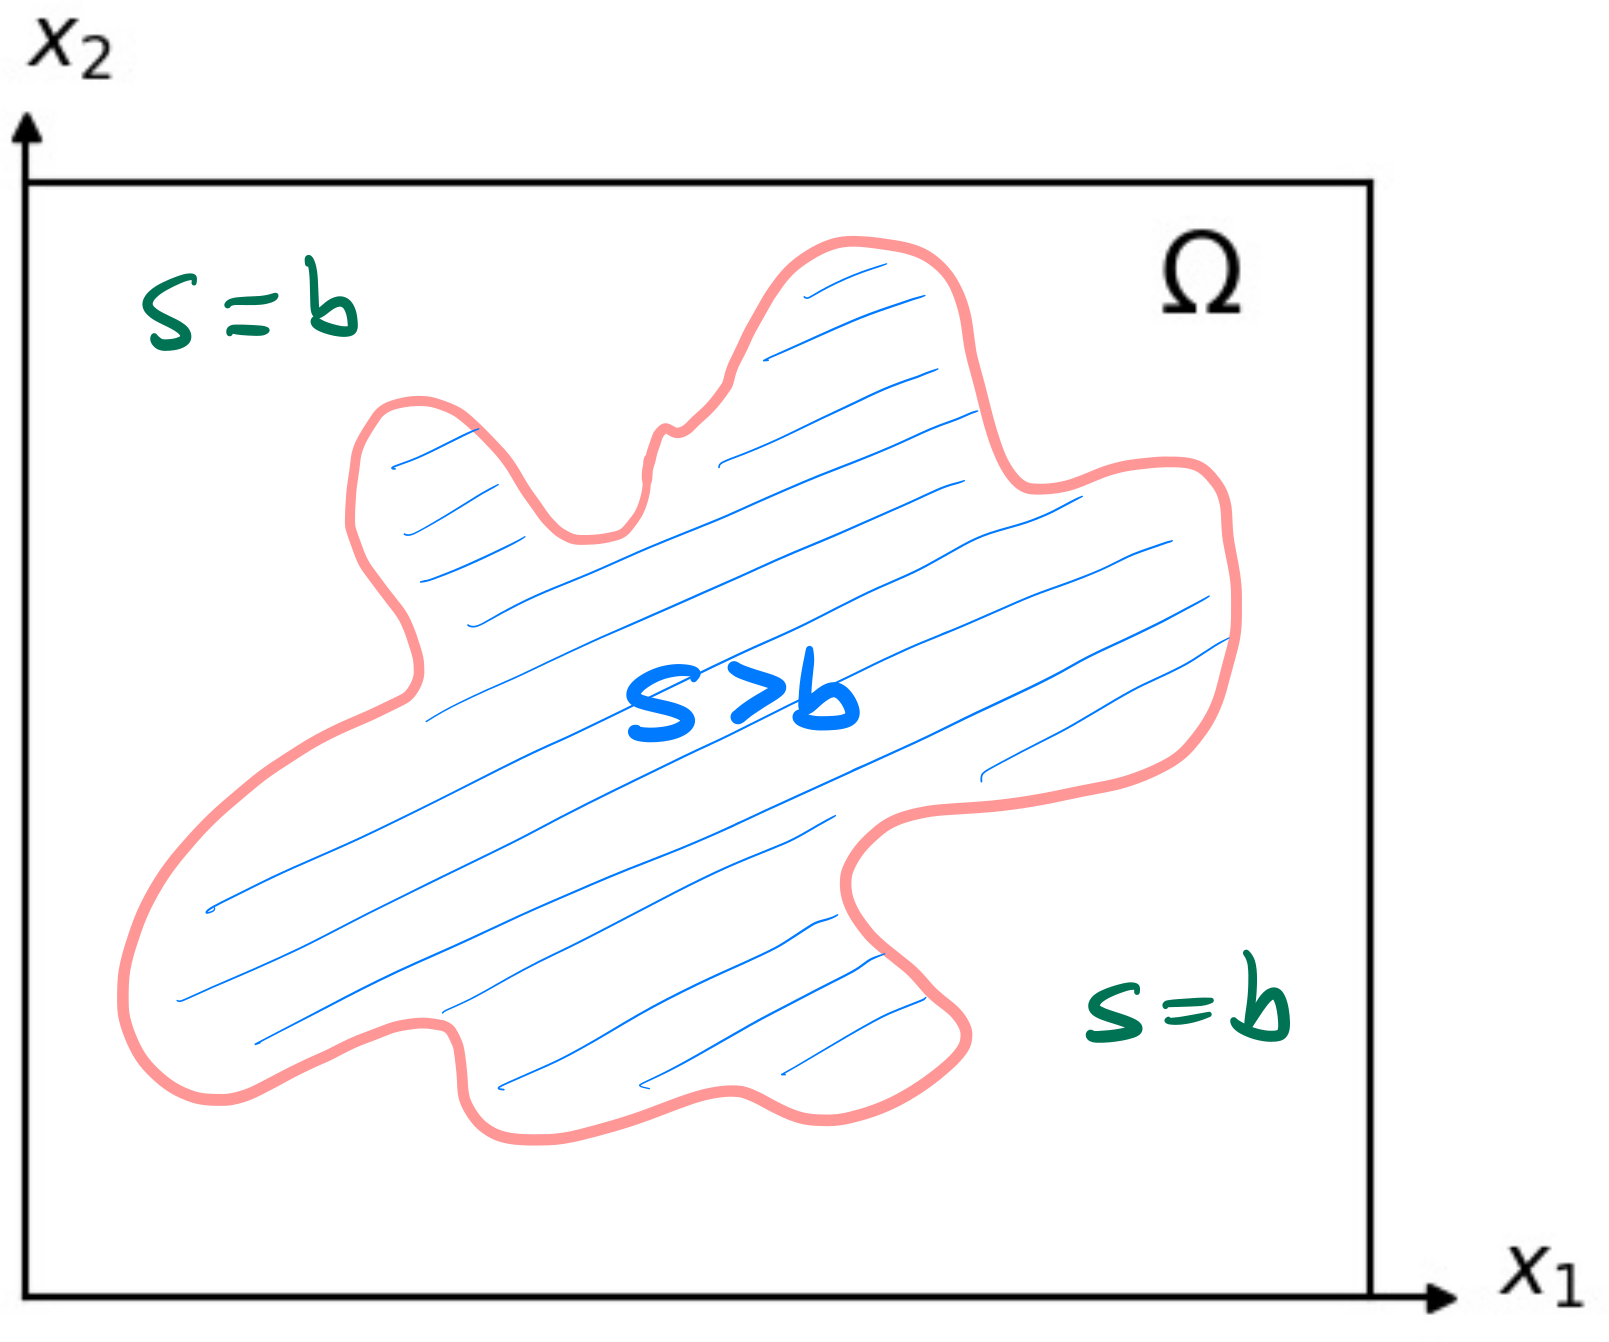
\includegraphics[width=0.37\textwidth]{mapplane}

\vspace{-40mm}

\begin{minipage}[t]{60mm}
{\small
\begin{itemize}
\item $\Omega \subset \RR^2$ fixed simulation domain
\item $x = (x_1,x_2) \in \Omega$
\item $a(t,x)$ surface mass balance (SMB)
\item $b(x)$ bed elevation
\item $s(t,x)$ \emph{solution} surface elevation
\item $\bn_s = (- \grad s,1)$ surface-normal vector
\item $\bu|_s(t,x)$ surface value of ice velocity, extended by zero to bare land
\end{itemize}
}
\end{minipage}

\begin{itemize}
\item nonlinear complementarity problem (NCP) in $[0,T] \times \Omega$:
\begin{align*}
s - b &\ge 0 &&\phantom{x} \\
\frac{\partial s}{\partial t} - \bu|_s \cdot \bn_s - a &\ge 0 \\
(s - b) \left(\frac{\partial s}{\partial t} - \bu|_s \cdot \bn_s - a\right) &= 0
\end{align*}
\end{itemize}
\end{frame}


\begin{frame}{the free-boundary problem for glacier surface elevation}

\begin{itemize}
\item surface kinematical equation (SKE) in glaciology:
   $$\frac{\partial s}{\partial t} - \bu|_s \cdot \bn_s - a = 0$$
\item our time-dependent, nonlinear complementarity problem (NCP) is the underlying \emph{free-boundary} meaning of the SKE:
\begin{align*}
s - b &\ge 0 &&\phantom{x} \\
\frac{\partial s}{\partial t} - \bu|_s \cdot \bn_s - a &\ge 0 \\
(s - b) \left(\frac{\partial s}{\partial t} - \bu|_s \cdot \bn_s - a\right) &= 0
\end{align*}

    \begin{itemize}
    \item[$\circ$] applies regardless of dynamical model within the ice
    \item[$\circ$] this NCP appears in (Calvo et al 2003), but only for shallow ice
    \end{itemize}
\item state-of-the-art numerically: first-order explicit time-stepping
\end{itemize}
\end{frame}


\begin{frame}{what is true within the ice?}

\hfill 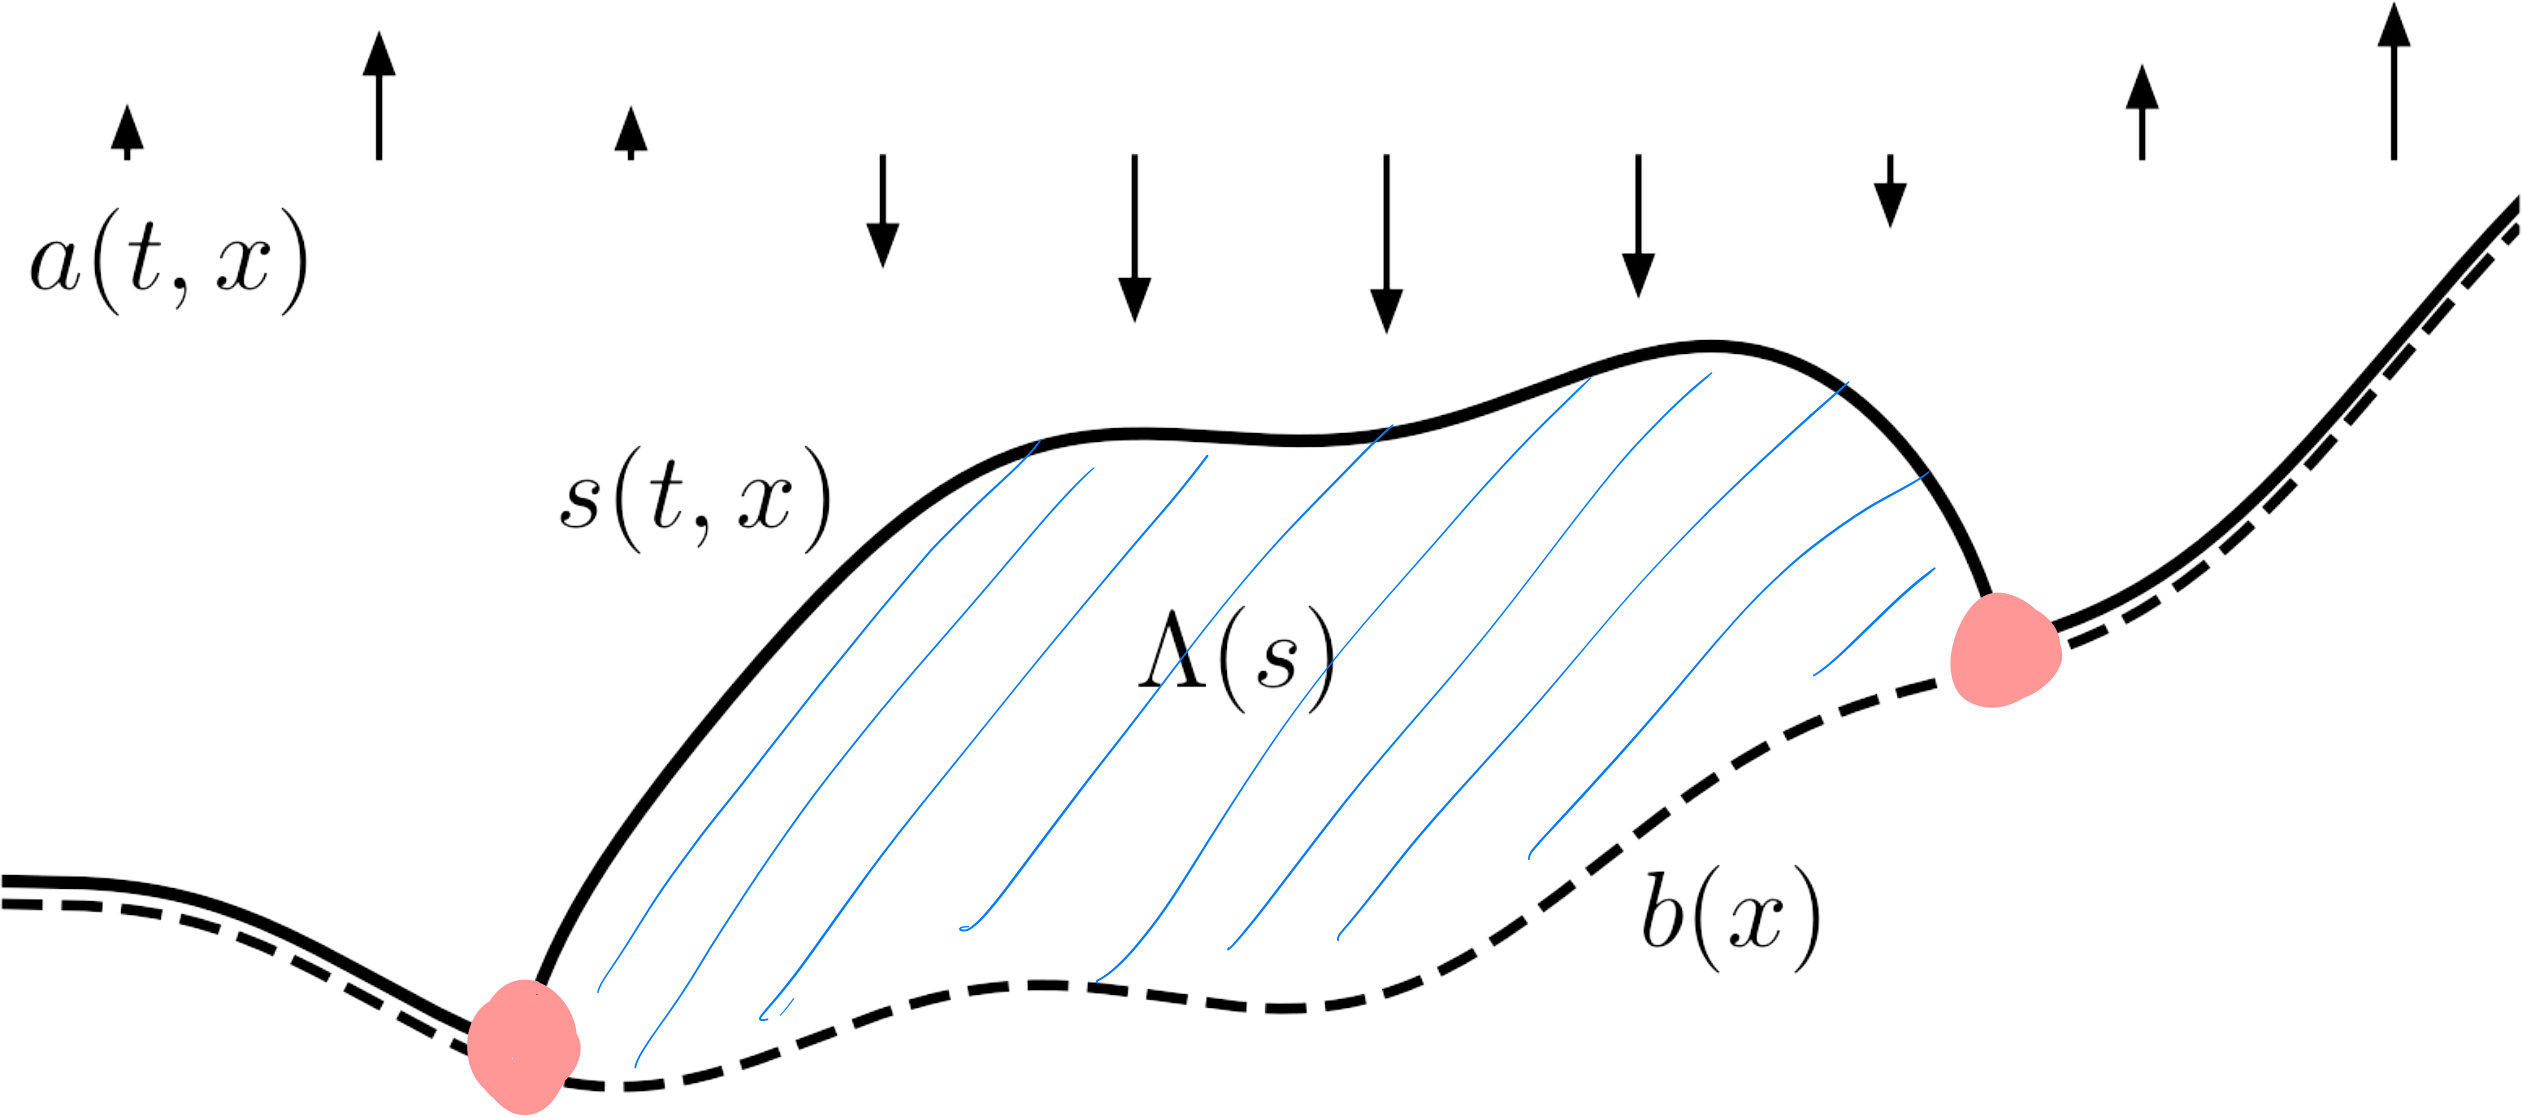
\includegraphics[width=0.55\textwidth]{stokesdomain}

\vspace{-5mm}

\begin{itemize}
\item fix $t$ and define:
    $$\Lambda(s) = \{(x,z)\,:\,b(x)<z<s(t,x)\} \qquad \subset \RR^3$$
\item Glen-Stokes equations in $\Lambda(s)$ with $\pp = (\nn + 1)/\nn \approx 4/3$:
\begin{align*}
- \nabla \cdot \left(2 \nu(D\bu)\, D\bu\right) + \nabla p &= \rhoi \bg  \\
\nabla \cdot \bu &= 0  \\
\nu(D\bu) &= \nu_0 |D\bu|^{\pp-2} && \quad {\scriptsize \leftarrow \text{needs regularization}}
\end{align*}

\vspace{-1mm}
\item boundary conditions:
\begin{align*}
&\left(2 \nu(D\bu) D\bu - pI\right) \bn_s = \bzero   && \where{on $\Gamma_s \subset \partial\Lambda(s)$} \\
&\bu  = \bzero \text{ } \,\text{or } \,f(\bu,D\bu)=0 && \where{on $\Gamma_b \subset \partial\Lambda(s)$}
\end{align*}
\end{itemize}
\end{frame}


\begin{frame}{\underline{the} standard model for glacier evolution}

\begin{align*}
s - b &\ge 0 & &\where{in $\Omega$} \\
\frac{\partial s}{\partial t} - \bu|_s \cdot \bn_s - a &\ge 0 \\
(s - b) \left(\frac{\partial s}{\partial t} - \bu|_s \cdot \bn_s - a\right) &= 0 \\
- \nabla \cdot \left(2 \nu_0 |D\bu|^{\pp-2}\, D\bu\right) + \nabla p &= \rhoi \bg && \where{in $\Lambda(s)$} \\
\nabla \cdot \bu &= 0 \\
\left(2 \nu(D\bu) D\bu - pI\right) \bn_s &= \bzero && \where{on $\Gamma_s \subset \partial\Lambda(s)$} \\
\bu  = \bzero \quad \text{or} \quad f(\bu,D\bu) &= 0 && \where{on $\Gamma_b \subset \partial\Lambda(s)$}
\end{align*}

\bigskip
\newtheorem*{smodel}{standard model}

\begin{smodel}
an NCP in $[0,T]\times \Omega$, for fixed $\Omega \subset \RR^2$, coupled to a Glen-Stokes problem within the ice, in $\Lambda(s) \subset \RR^3$
\end{smodel}
\end{frame}


\begin{frame}{the standard model wants ``fully-implicit'' time-stepping}

\begin{center}
FIXME %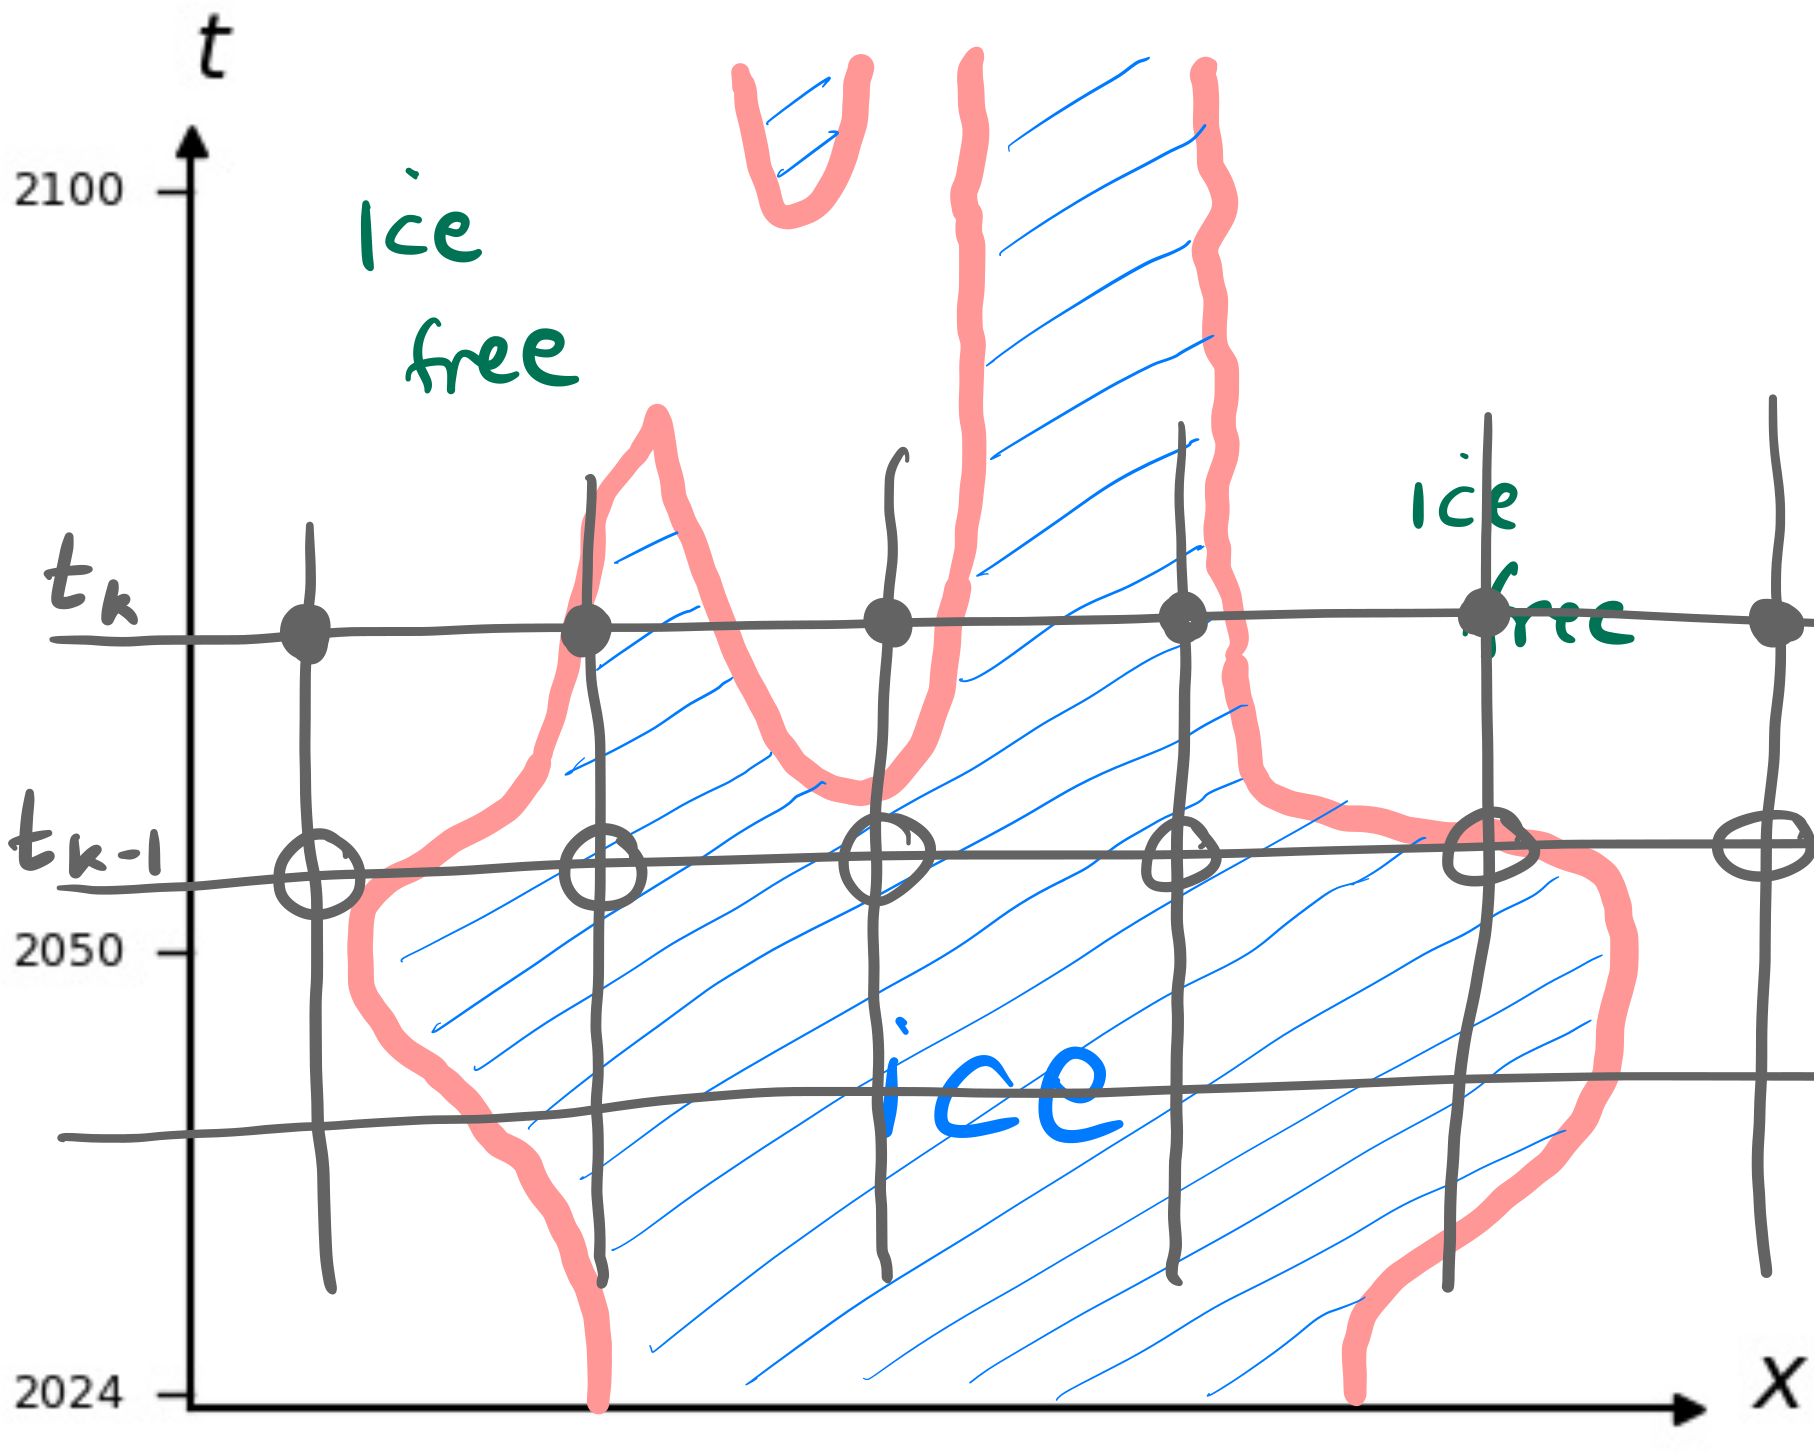
\includegraphics[width=0.6\textwidth]{implicitstep}
\end{center}

\bigskip
\begin{block}{standard model as a dynamical system}
an inequality-constrained \textbf{differential algebraic system} in $\infty$ dimensions
\end{block}
\end{frame}


\AtBeginSection[]
{
  \begin{frame}<beamer>
    \frametitle{Outline}
    \tableofcontents[currentsection,hideallsubsections]
  \end{frame}
}


\section{well-posed implicit steps?}

\begin{frame}{implicit time-step problem is a variational inequality}

\begin{itemize}
\item weak form of time-discretized NCP; details found in preprint\footnote{Bueler (2024). \emph{Surface elevation errors in finite element Stokes models for glacier evolution}, \href{https://www.arxiv.org/abs/2408.06470}{arxiv 2408.06470}}
\item $\cX$ denotes Banach space of elevation functions on $\Omega$; $b\in\cX$
\item for $\Delta t > 0$ define:

\vspace{-7mm}
\begin{align*}
\cK &= \{r \in \cX\,:\, r \ge b \,\text{ a.e. } \Omega\} \\
\ell^k(x) &= s(t_{k-1},x) + \int_{t_{k-1}}^{t_k} a(t,x)\,dt \\
F(s)[q] &= \int_\Omega (s - \Delta t\,\bu|_s \cdot \bn_s) q 
\end{align*}
\end{itemize}

\medskip
\begin{definition}
the \emph{backward Euler time-step problem}, for $t_k \in [0,T]$, is to find the surface elevation $s \approx s(t_k,x) \in \cK$ solving the variational inequality (VI)
$$F(s)[r-s] \ge \ell^k[r-s] \quad \text{for all } r \in \cK$$
\end{definition}

\bigskip
\end{frame}


\begin{frame}{well-posedness is only conjectural}

\hfill 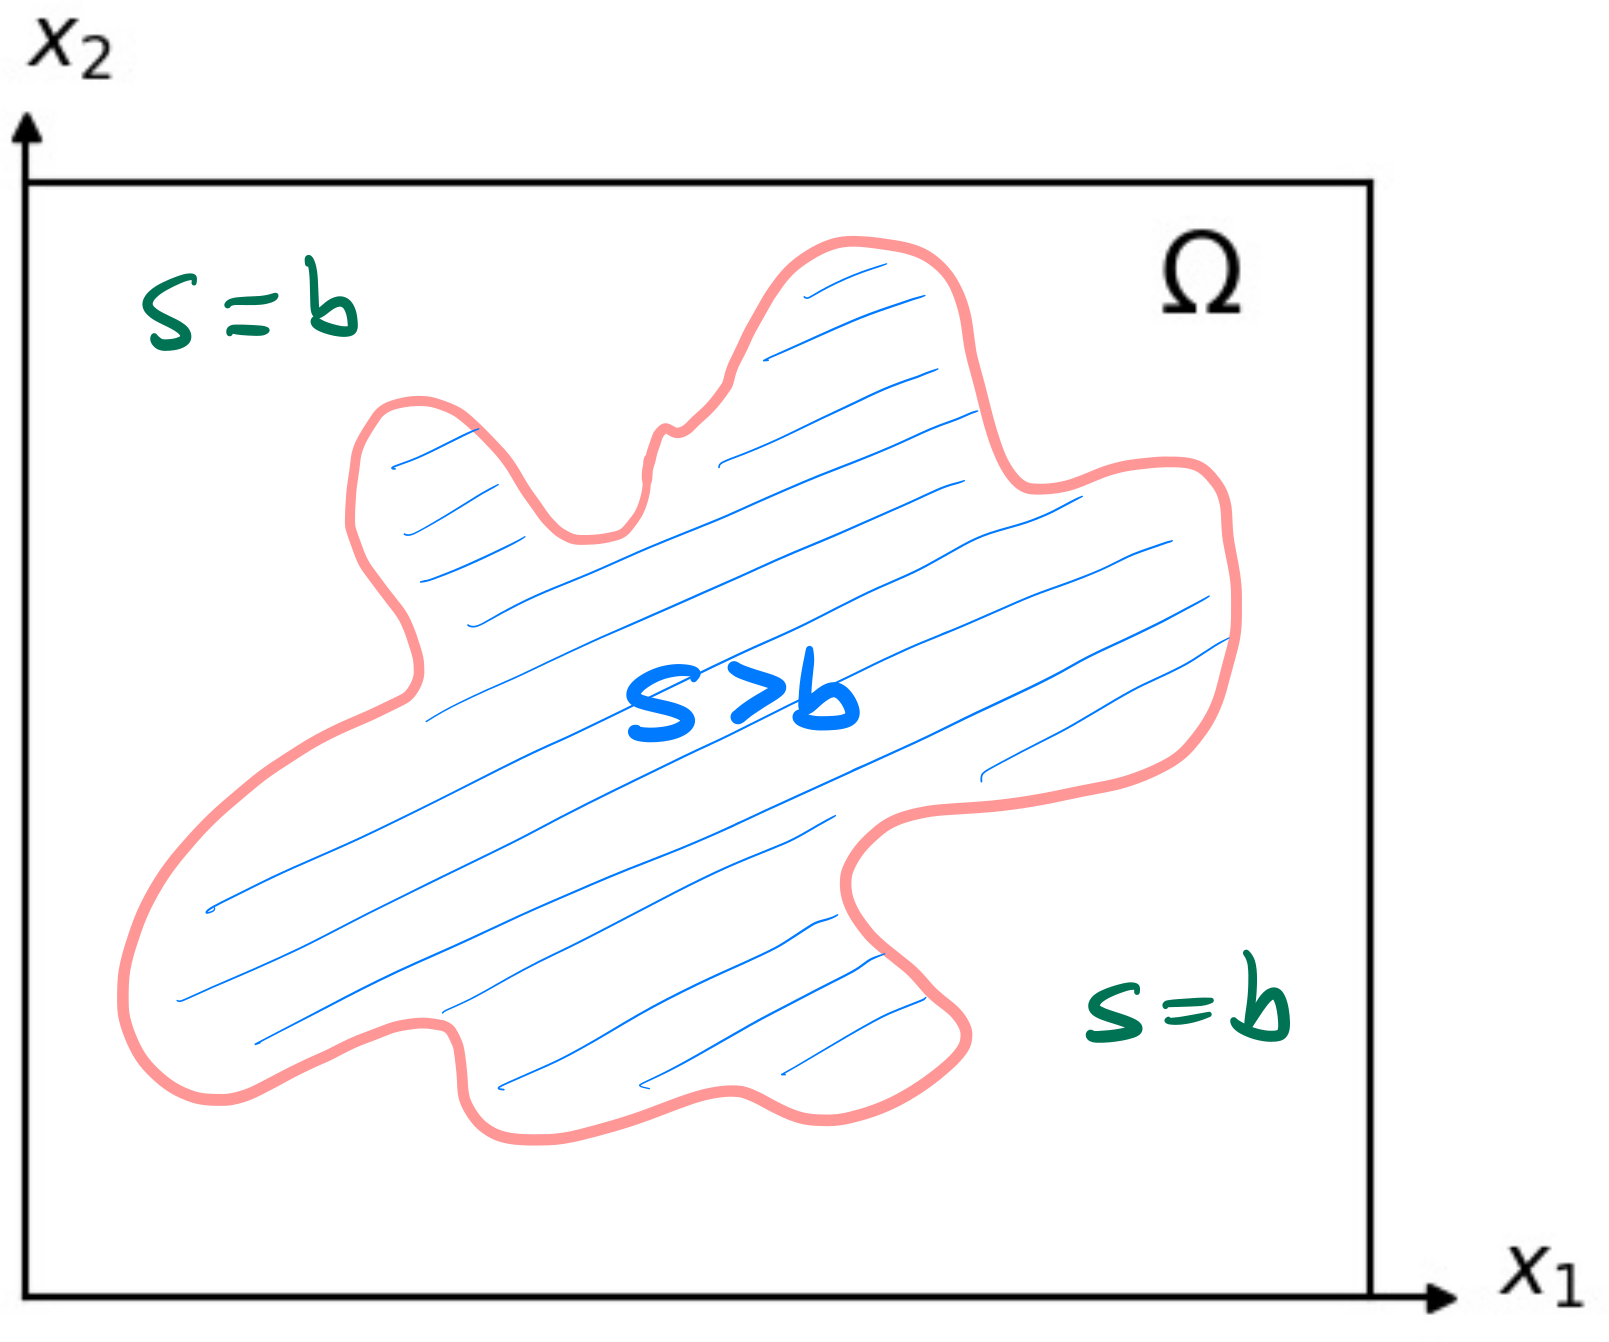
\includegraphics[width=0.35\textwidth]{mapplane}

\begin{conjecture}[B '24]
for some $\qq>2$, with $\cX = W^{1,\qq}(\Omega)$, and defining the admissible surface elevation subset
    $$\cK = \{r \ge b\} \subset \cX,$$
the backward Euler time-step VI problem,
    $$F(s)[r-s] \ge \ell^k[r-s] \quad \text{for all } r \in \cK,$$
is well-posed for $s\in\cK$
\end{conjecture}
\end{frame}


\begin{frame}{what's behind the conjecture? 1}

\begin{center}
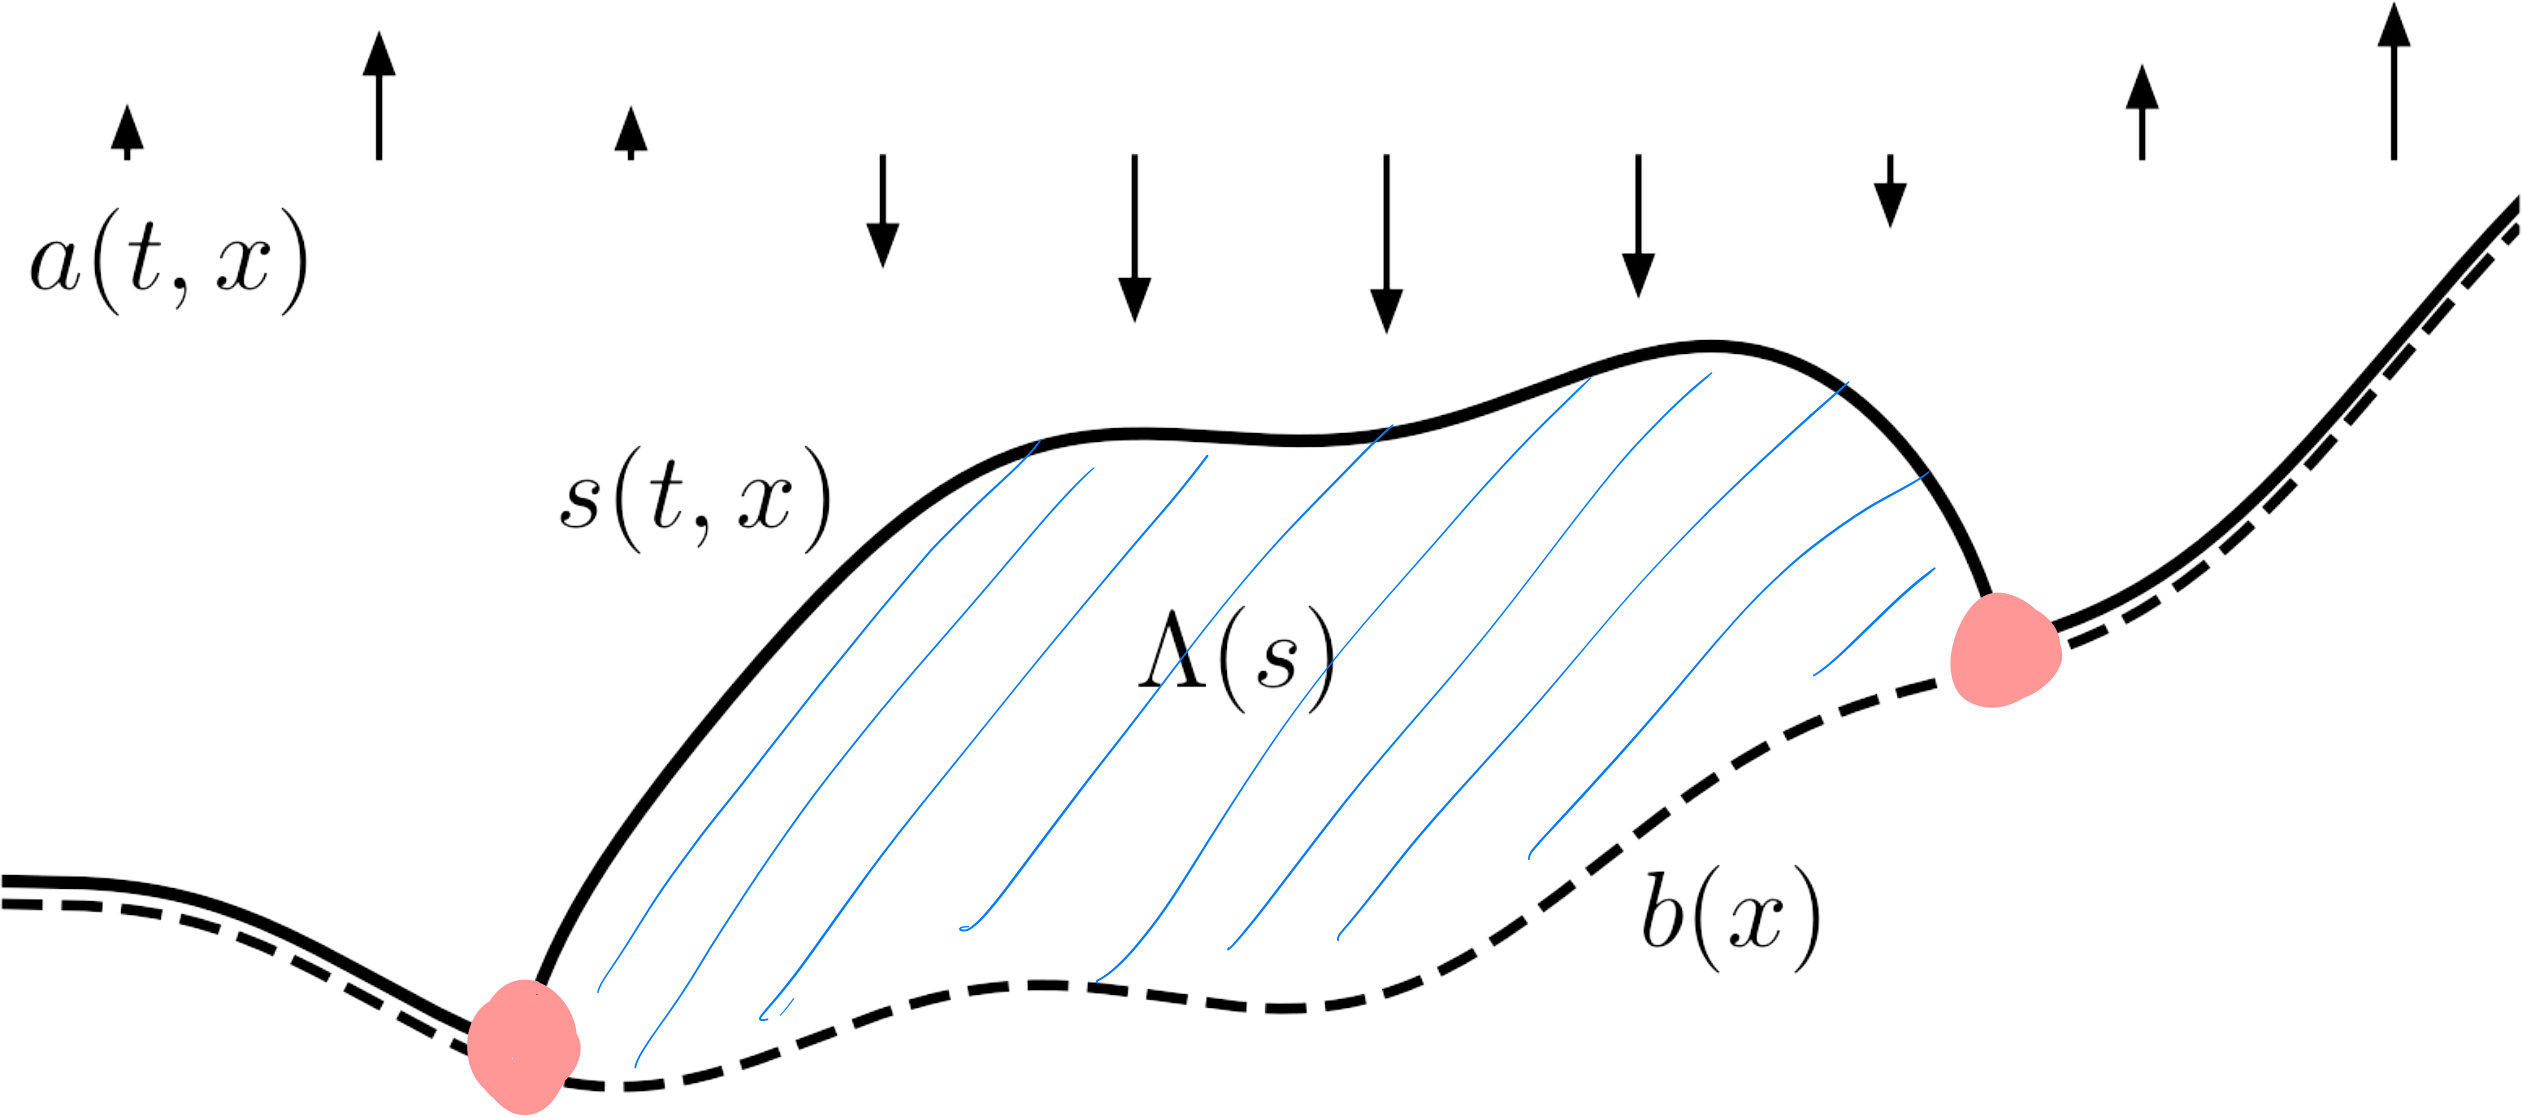
\includegraphics[width=0.6\textwidth]{stokesdomain}
\end{center}

\begin{theorem}[Jouvet \& Rappaz, 2011]
over a fixed domain $\Lambda$, the Glen-Stokes problem
\begin{align*}
- \nabla \cdot \left(2 \nu_0 |D\bu|^{\pp-2}\, D\bu\right) + \nabla p &= \rhoi \bg && \where{in $\Lambda$} \\
\nabla \cdot \bu &= 0 \\
\left(2 \nu(D\bu) D\bu - pI\right) \bn_s &= \bzero && \where{on $\Gamma_s \subset \partial\Lambda$} \\
\bu  = \bzero \quad \text{or} \quad f(\bu,D\bu) &= 0 && \where{on $\Gamma_b \subset \partial\Lambda$}
\end{align*}
is well-posed for $(\bu,p) \in W^{1,\pp}_0(\Omega;\RR^3) \times L^{\pp'}(\Omega)$
\end{theorem}
\end{frame}


\begin{frame}{what's behind the conjecture? 2}

\bigskip
\begin{center}
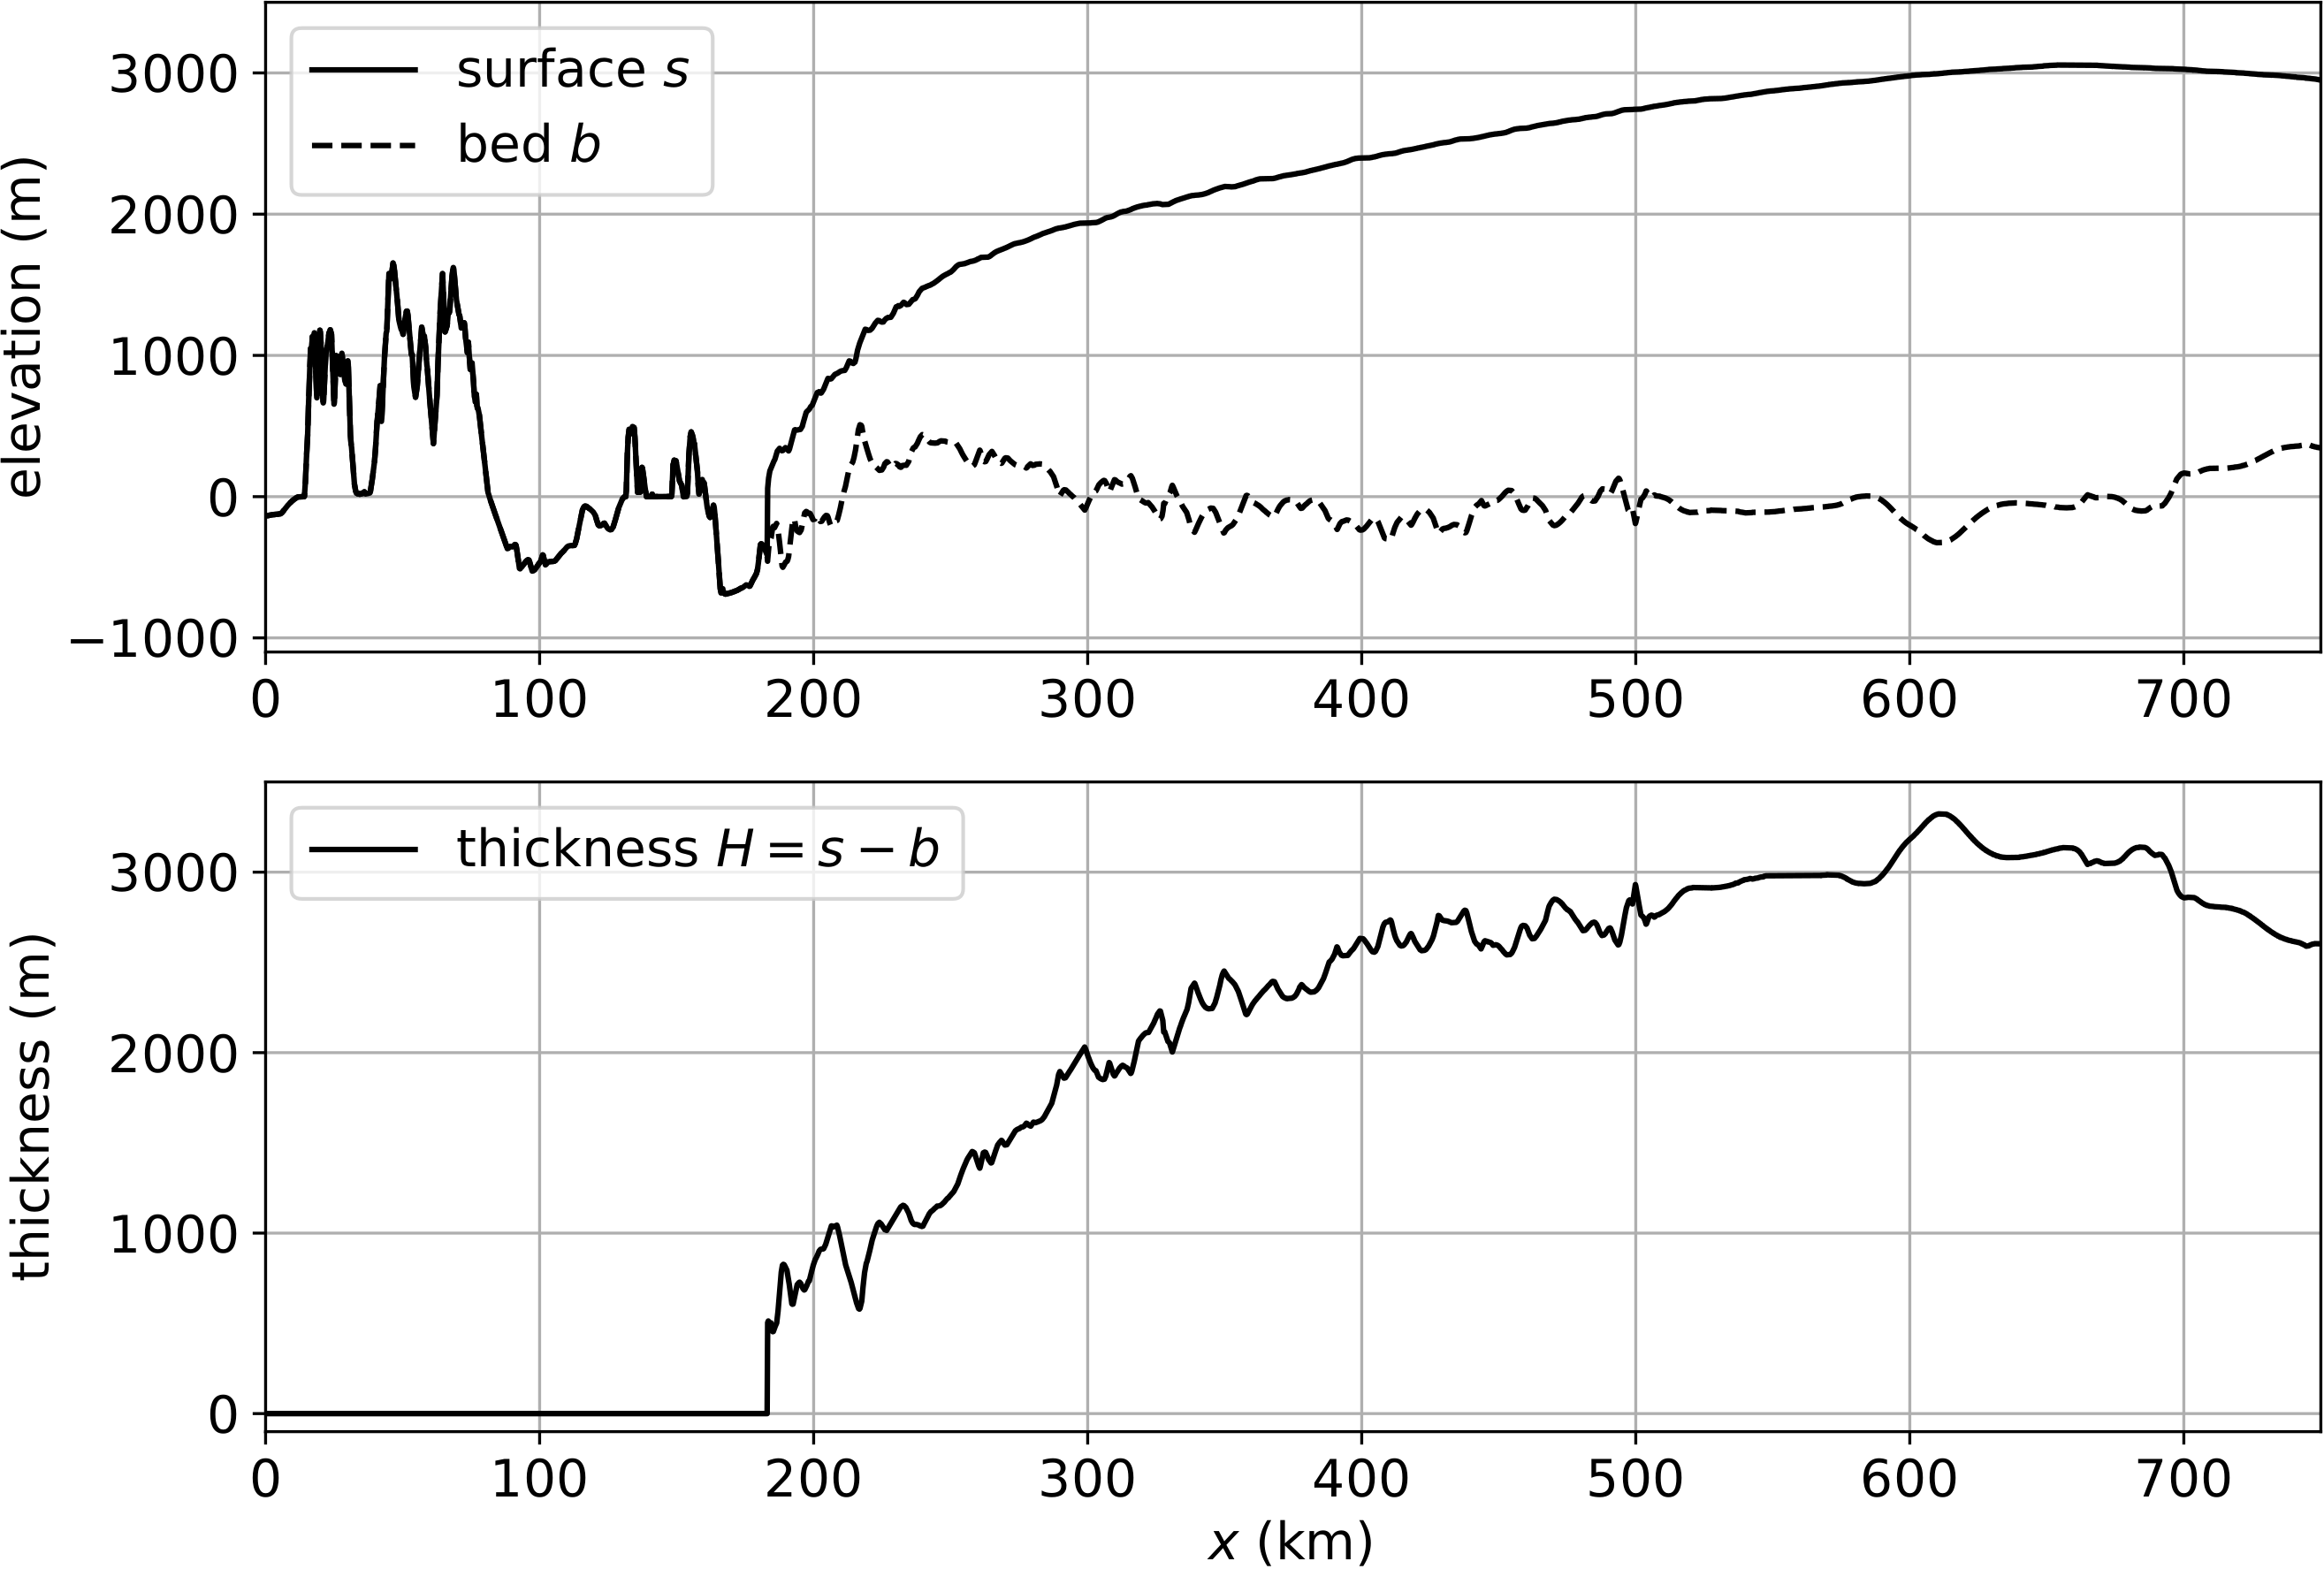
\includegraphics[width=0.75\textwidth]{giscross}
\end{center}

\begin{itemize}
\item question: use ice surface elevation $s$ or thickness $H = s - b$ for geometry in the standard model?
\item answer: prefer $s$ for smoothness reasons
\end{itemize}
\end{frame}


\begin{frame}{what's behind the conjecture? 3}

\begin{center}
\begin{tikzpicture}[scale=1.0]
  \node (wedge) {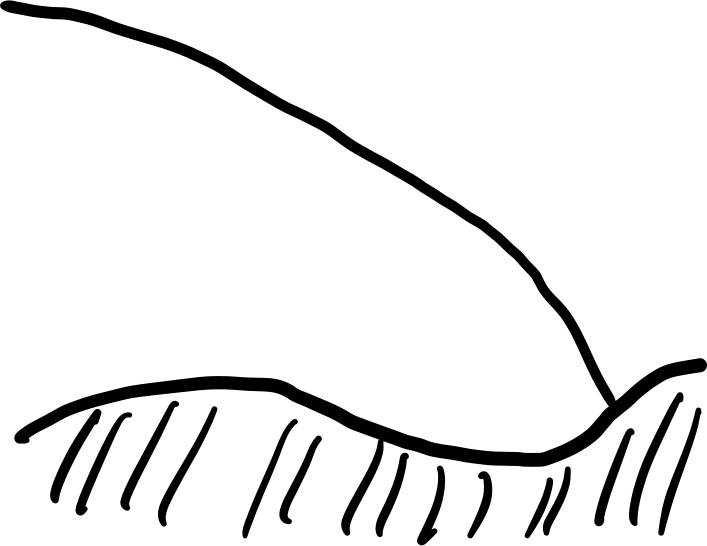
\includegraphics[width=30mm]{wedge.png}} node[xshift=-4mm, yshift=1mm] at (wedge.center) {{\small \emph{ice}}};
  \node[right= 5mm of wedge] (unbounded) {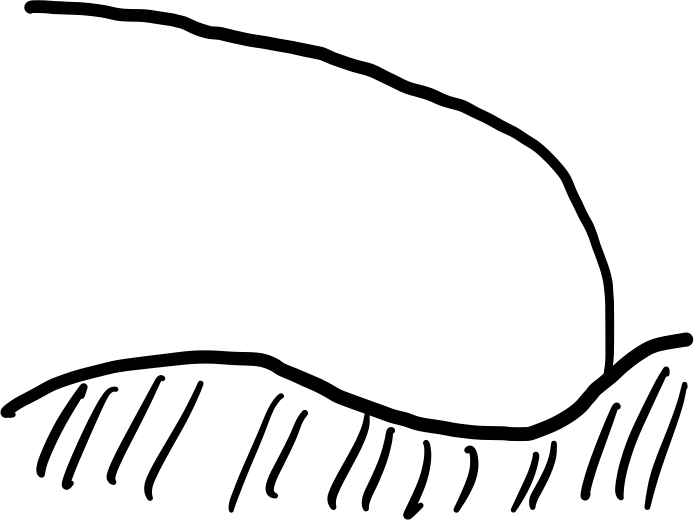
\includegraphics[width=30mm]{unbounded.png}} node[xshift=-2mm, yshift=1mm] at (unbounded.center) {{\small \emph{ice}}};
  \node[right= 5mm of unbounded] (realistic) {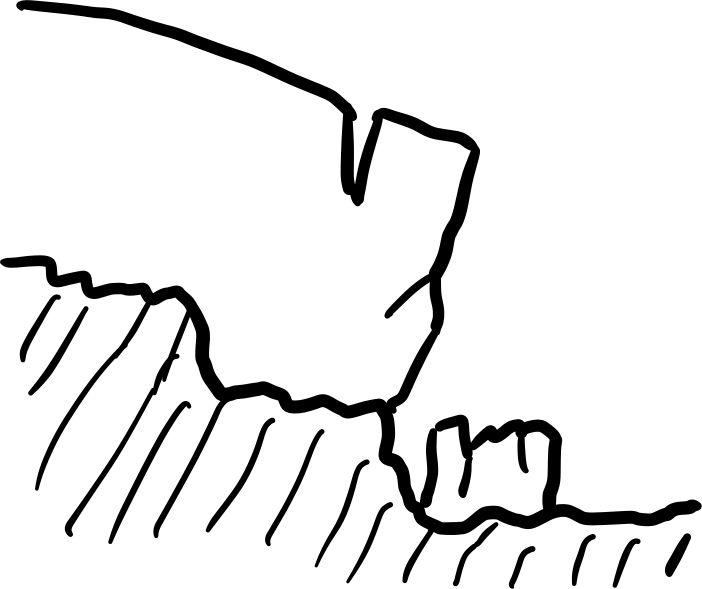
\includegraphics[width=30mm]{realistic.png}} node[xshift=-6mm, yshift=4mm] at (realistic.center) {{\small \emph{ice}}};
\end{tikzpicture}
\end{center}

\begin{itemize}
\item the conjecture is that $s$ exists in $\cX = W^{1,\qq}(\Omega)$ for some $\qq>2$
\item however, margin shape of glaciers is a hard modeling problem
\end{itemize}
\end{frame}


\begin{frame}{what's behind the conjecture? 4}

\bigskip
\begin{conjecture}[actual; B '24]
For $s \in \cK = \{r \ge b\} \subset \cX = W^{1,\qq}(\Omega)$, for some $\qq>2$, let $\Lambda(s) = \{b<z<s\} \subset \RR^3$, and suppose $\bu$ solves Glen-Stokes over $\Lambda(s)$.  Define
	$$\Phi(s) = - \bu|_s \cdot \bn_s,$$
a map $\Phi:\cK \to \cX'$.  Then $\Phi$ is $\qq$-coercive: there is $\alpha>0$ so that
	$$\left(\Phi(s) - \Phi(r)\right)[r-s] \ge \alpha \|r-s\|_\cX^\qq \qquad \text{for all } r,s\in\cK$$
\end{conjecture}

\bigskip
\footnotesize
\noindent \textbf{numerical evidence?}

\begin{itemize}
\item from surface elevation samples $r,s$, compute

numerical ratios $\displaystyle \frac{(\Phi(r)-\phi(s))[r-s]}{\|r-s\|_\cX^\qq}$
\end{itemize}

\vspace{-22mm}
FIXME %\hfill 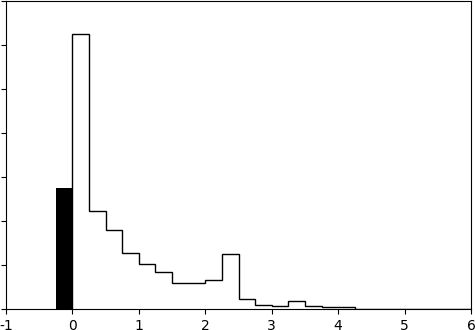
\includegraphics[width=0.3\textwidth]{smoothratios} \qquad
\end{frame}


\section{application: surface elevation error bound}

\begin{frame}{FE method}

\begin{center}
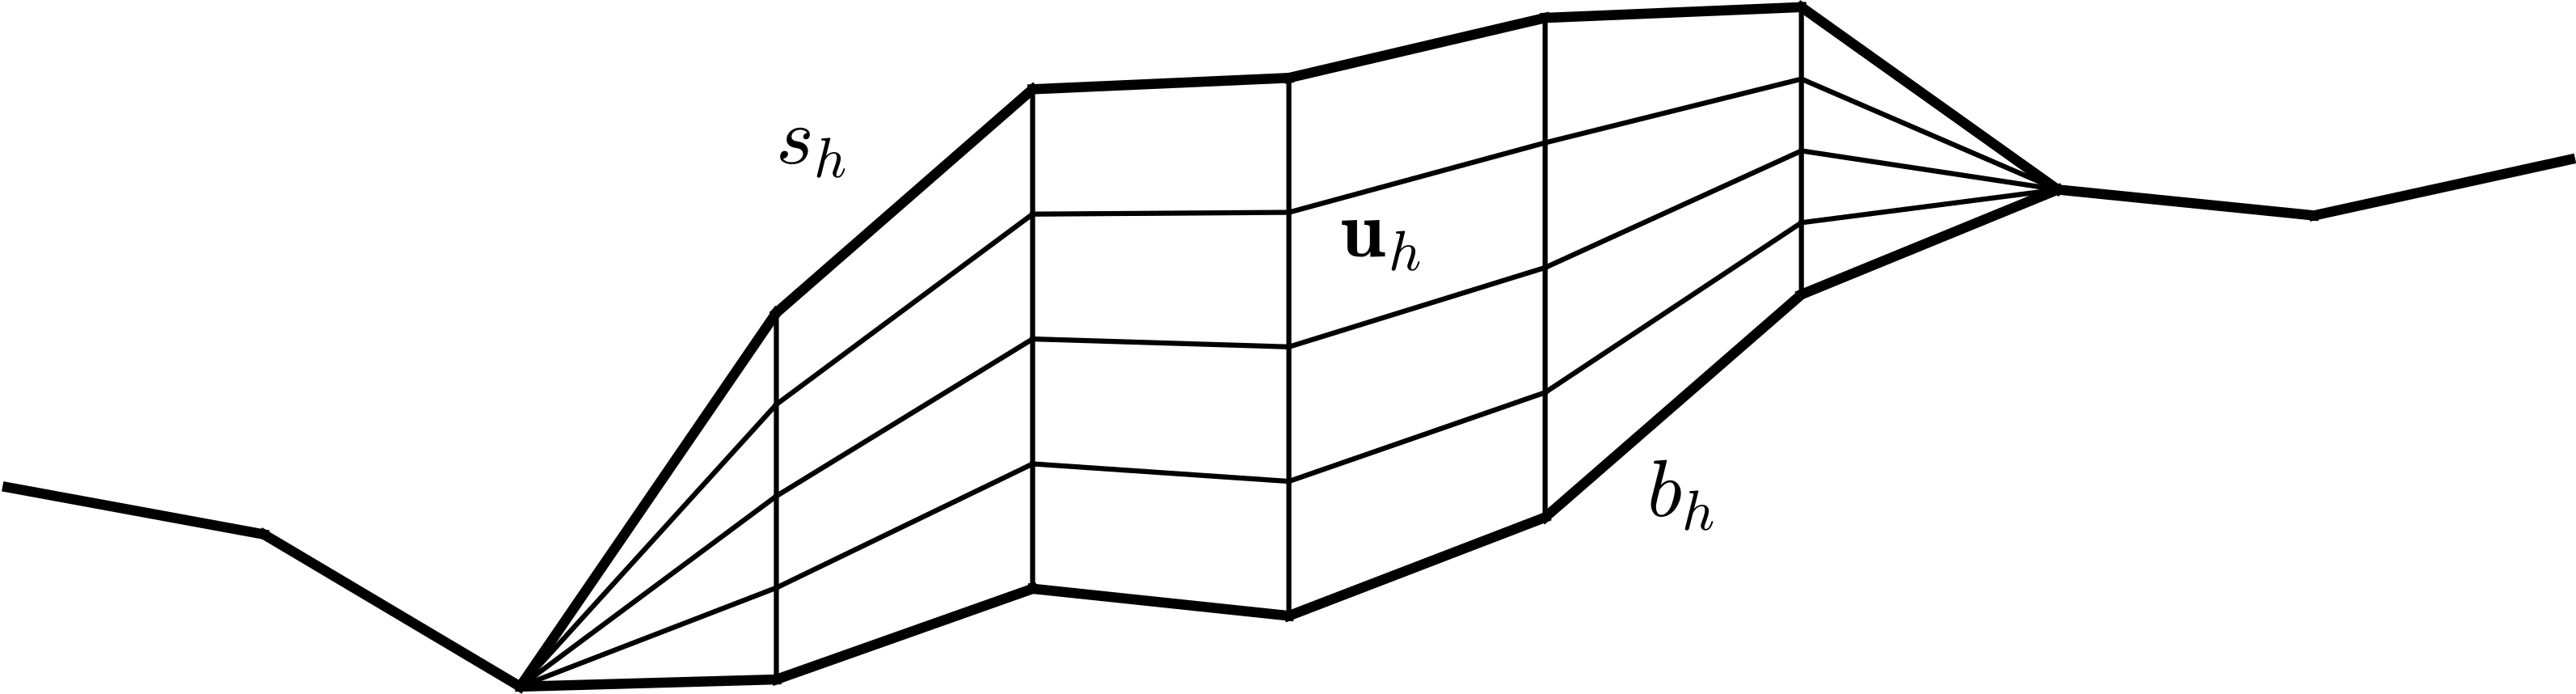
\includegraphics[width=0.7\textwidth]{extruded}
\end{center}

\begin{cproblem}
find $s\in\cK = \{r \ge b\}$ which solves the backward-Euler step VI:
   $$F(s)[r-s] \ge \ell^k[r-s] \quad \text{for all } r \in \cK$$
\end{cproblem}

\begin{itemize}
\item proposed FE spaces:
   \begin{itemize}
   \item[$\circ$] $b_h,s_h \in P_1$
   \item[$\circ$] $\bu_h,p_h \in P_2 \times P_1$, on an extruded mesh \hfill {\scriptsize $\leftarrow$ one possibility}
   \end{itemize}
\item FE method for $s_h\in\cK_h = \{r_h \ge b_h\}$:
   $$F_h(s_h)[r_h-s_h] \ge \ell^k[r_h-s_h] \quad \text{for all } r_h \in \cK_h$$

   \begin{itemize}
   \item[$\circ$] mostly conforming, especially if one pretends $b_h=b$
   \end{itemize}
\end{itemize}

\phantom{x}
\end{frame}


\begin{frame}{implementation \alert{\dots in progress}}

\begin{itemize}
\item extruded-mesh Stokes solver infrastructure: \href{https://github.com/bueler/stokes-extrude}{github.com/bueler/stokes-extrude}
\item solver in Firedrake/PETSc:
    \begin{itemize}
    \item[$\circ$] VI-adapted, reduced-space Newton method
    \item[$\circ$] for admissible surface elevation iterates $s_h^{(j)} \ge b_h$, \alert{each residual evaluation $F(s_h^{(j)})$ requires solving the Glen-Stokes model on $\Lambda(s_h^{(j)})$ to get $\bu_h^{(j)}$}
    \end{itemize}
\item accelerate using new FASCD nonlinear multigrid scheme (Bueler \& Farrell, 2024), using above solver as the smoother
\end{itemize}

\bigskip
\end{frame}


\begin{frame}{error theorem for a backward Euler step}

\noindent 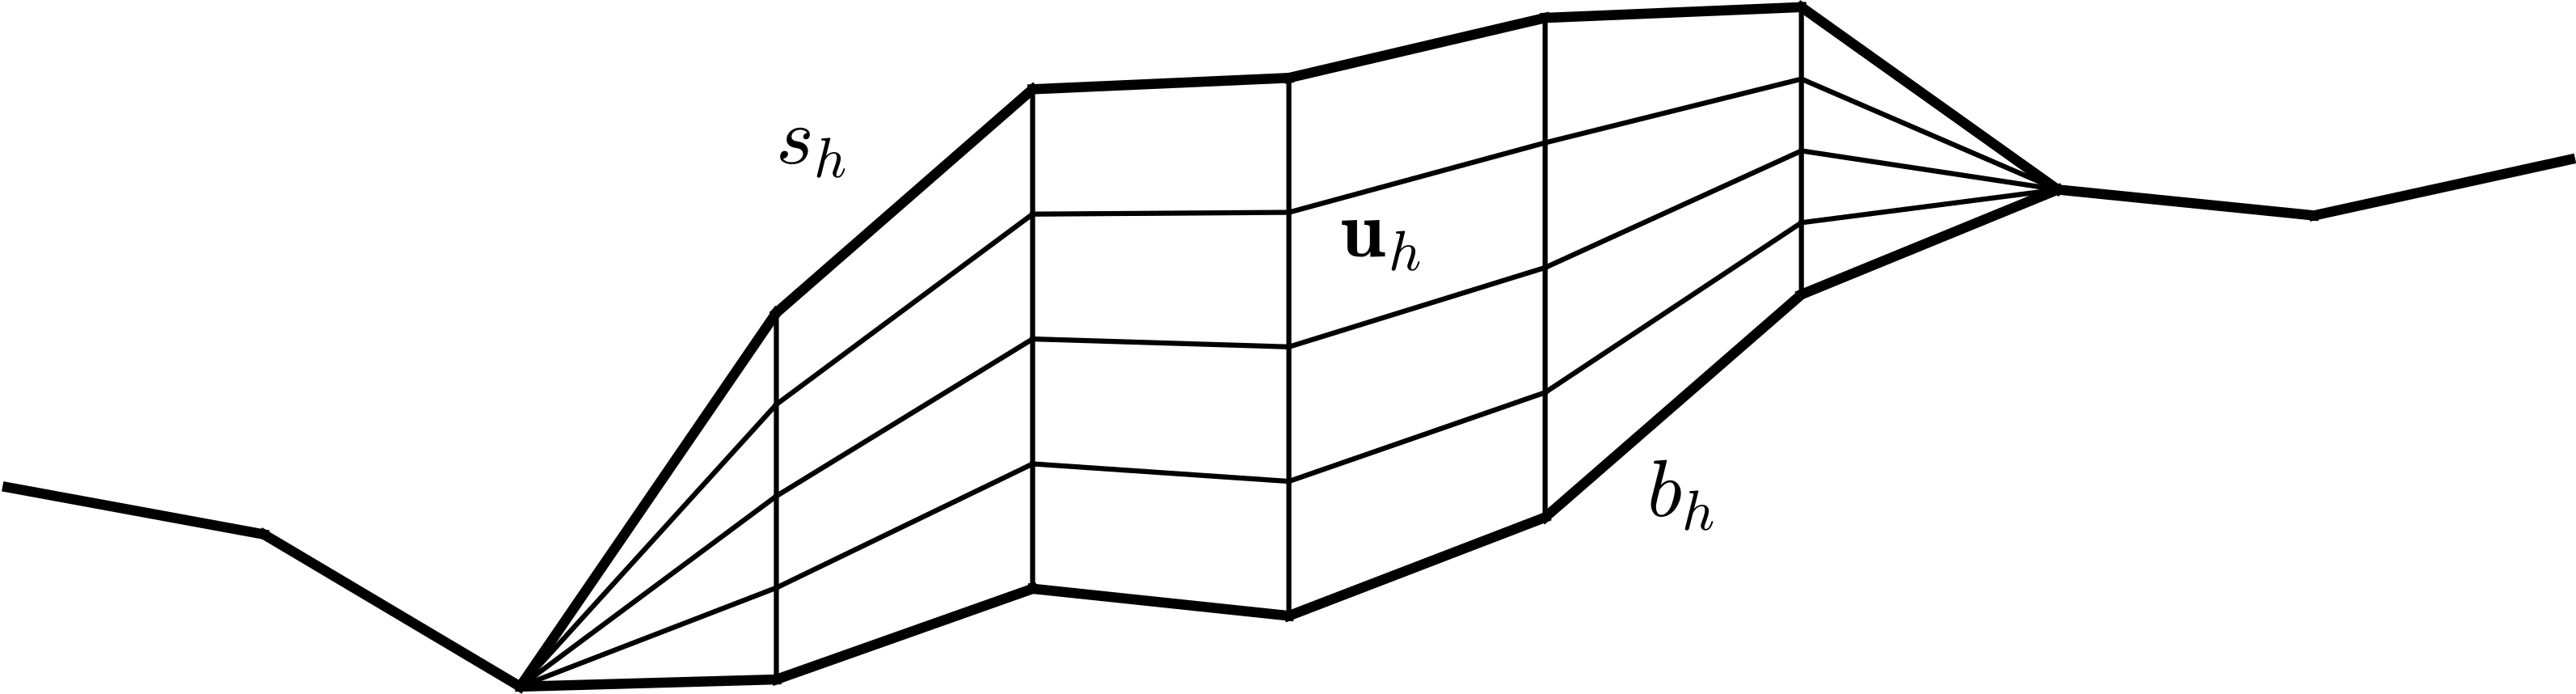
\includegraphics[width=0.6\textwidth]{extruded} \hfill 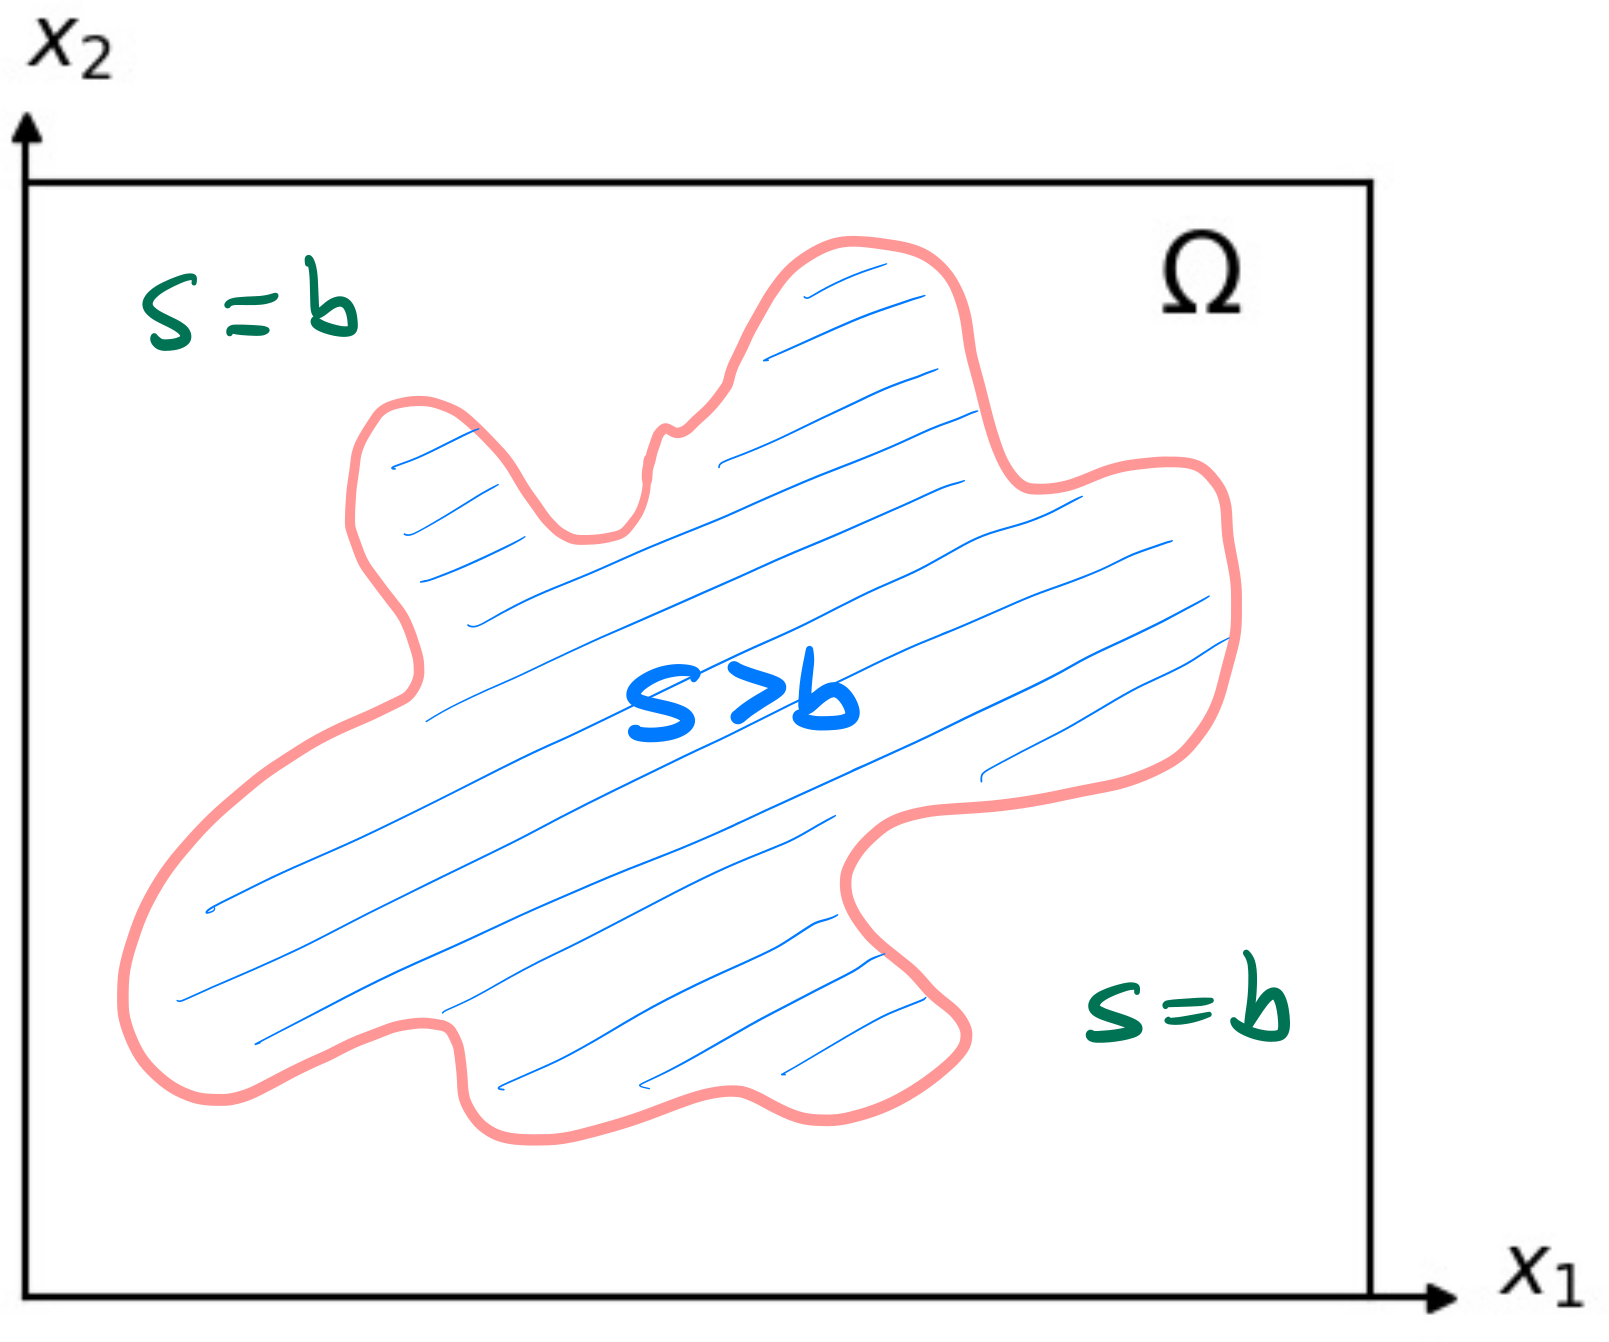
\includegraphics[width=0.23\textwidth]{mapplane}

\medskip
\begin{theorem}[B '24]
Make assumptions sufficient for well-posedness.  Let $\Omega_A(s)$ be  the exact active set, and $\Pi_h$ the interpolation into $\cK_h = \{r_h \ge b_h\}$.  Then the FE error in the new ($t_k$) surface elevation is bounded by 3 terms:
\begin{align*}
\|s_h-s\|_{W^{1,\qq}}^\qq &\le \, \frac{c_1}{\Delta t} \int_{\Omega_A(s)} (b - \ell^k) (b_h - b) \\
   &\quad\, + C(s_h) \big\|\bu_h - \bu\big\|_{W^{1,\pp}} \\
   &\quad\, + c_0 \|\Pi_h(s) - s\|_{W^{1,\qq}}^{\qq'}
\end{align*}
\end{theorem}

\noindent \emph{Proof.} Make the Falk (1974) technique for VIs fully nonlinear. \qed
\end{frame}


\begin{frame}{summary}
\begin{itemize}
\item implicit time-stepping makes sense for geometry-evolving, Stokes models for glaciers
    \begin{itemize}
    \item[$\circ$] both a differential-algebraic system and a free-boundary problem
    \end{itemize}
\item \textbf{conjecture.} for some $\qq>2$, the surface motion $-\bu|_s\cdot \bn_s$ from the Glen-Stokes problem is $\qq$-coercive over admissible $s\in W^{1,\qq}(\Omega)$
\item \textbf{theorem.} supposing $\qq$-coercivity, each continuous-space, backward Euler time step problem is well-posed
\item \textbf{theorem.} supposing well-posedness, the surface elevation FE error is bounded by a sum of 3 terms:
    \begin{enumerate}
    \item discretizing the bed elevation ($b_h$ versus $b$)
    \item numerically solving the Stokes equations ($\bu_h$ versus $\bu$)
    \item Cea's lemma for the surface elevation ($s_h$ versus $\Pi_h(s)$) \strut
    \end{enumerate}
\end{itemize}
\end{frame}


\begin{frame}{references}

{\footnotesize % inputed at end of slides.tex

\newcommand{\sdoi}[1]{\,{\scriptsize \href{https://doi.org/#1}{doi:#1}}}
\newcommand{\surl}[2]{\,{\scriptsize \href{#1}{#2}}}

\begin{itemize}
%\item E.~Bueler (2021). \emph{Conservation laws for free-boundary fluid layers}, SIAM J.~Appl.~Math.~81 (5), 2007--2032 \sdoi{10.1137/20M135217X}
%\item E.~Bueler (2022). \emph{Performance analysis of high-resolution ice-sheet simulations}, J.~Glaciol.~69 (276), 930--935 \sdoi{10.1017/jog.2022.113}
%\item E.~Bueler \& P.~Farrell (2024).  \emph{A full approximation scheme multilevel method for nonlinear variational inequalities}, SIAM J.~Sci.~Comput.~46 (4), \sdoi{10.1137/23M1594200}
\item E.~Bueler (2024). \emph{Surface elevation errors in finite element {S}tokes models for glacier evolution}, submitted \surl{https://arxiv.org/abs/2408.06470}{arxiv:2408.06470}
\item N.~Calvo and others (2003). \emph{On a doubly nonlinear parabolic obstacle problem modelling ice sheet dynamics}, SIAM J.~Appl.~Math.~63 (2), 683--707 \sdoi{10.1137/S0036139901385345}
%\item T.~Isaac, G.~Stadler, \& O.~Ghattas (2015). \emph{Solution of nonlinear Stokes equations \dots ice sheet dynamics}, SIAM J.~Sci.~Comput., 37 (6), B804--B833 \sdoi{10.1137/140974407}
%\item G.~Jouvet \& E.~Bueler (2012). \emph{Steady, shallow ice sheets as obstacle problems: well-posedness and finite element approximation}, SIAM J.~Appl.~Math.~72 (4), 1292--1314 \sdoi{10.1137/110856654}
\item G.~Jouvet \& J.~Rappaz (2011). \emph{Analysis and finite element approximation of a nonlinear stationary {S}tokes problem \dots}, Adv.~Numer.~Analysis 2011 (164581) \sdoi{10.1155/2011/164581}
%\item A.~L{\"o}fgren, J.~Ahlkrona \& C. Helanow (2022). \emph{Increasing stable time-step sizes of the free-surface problem arising in ice-sheet simulations},~J. Comput. Phys.: X 16 (100114) \sdoi={10.1016/j.jcpx.2022.100114}
\end{itemize}
}
\end{frame}

\end{document}
